\documentclass[conference]{IEEEtran}
\IEEEoverridecommandlockouts
\usepackage{cite}
\usepackage{amsmath,amssymb,amsfonts}
\usepackage{algorithmic}
\usepackage{algorithm}
\usepackage{graphicx}
\usepackage{textcomp}
\usepackage{xcolor}
\usepackage{array}
\usepackage{booktabs}
\usepackage{multirow}
\usepackage{url}
\usepackage{tikz}
\usetikzlibrary{shapes.geometric, arrows.meta, positioning, fit, backgrounds, calc}
\usepackage{pgfplots}
\pgfplotsset{compat=1.18}

% TikZ styles
\tikzset{
  proc/.style={rectangle, rounded corners=3pt, draw=black, fill=blue!12, 
               text width=2.0cm, align=center, minimum height=0.55cm, font=\scriptsize},
  data/.style={rectangle, draw=black, fill=orange!18, 
               text width=2.0cm, align=center, minimum height=0.55cm, font=\scriptsize},
  decision/.style={diamond, draw=black, fill=yellow!20, 
                   text width=1.5cm, align=center, inner sep=1pt, font=\scriptsize},
  storage/.style={cylinder, shape border rotate=90, draw=black, fill=green!15,
                  text width=1.7cm, align=center, minimum height=0.6cm, font=\scriptsize},
  arrow/.style={-Stealth, thick},
  label/.style={font=\tiny, midway, fill=white, inner sep=1pt},
}

\def\BibTeX{{\rm B\kern-.05em{\sc i\kern-.025em b}\kern-.08em
    T\kern-.1667em\lower.7ex\hbox{E}\kern-.125emX}}

\begin{document}

\title{Label Padhega: A Multi-Engine AI System for\\Real-Time Food Label Analysis in the Indian Context}

\author{
\IEEEauthorblockN{[Author Name(s)]}
\IEEEauthorblockA{
\textit{[Department, Institution]}\\
[City, India]\\
[email@institution.ac.in]
}
}

\maketitle

% ─────────────────────────────────────────────────────────────────────────────
\begin{abstract}
Ultra-processed food consumption in India has risen sharply: ICMR-NIN data show that
hidden sugar, sodium, and synthetic additives account for an estimated 56.4\% of
preventable non-communicable disease (NCD) burden in the country, yet fewer than
9\% of Indian consumers report reading ingredient labels before purchase \cite{fssai_survey}.
Existing label-reading tools are either generic (not India-specific), paywalled,
or produce a single opaque numeric verdict with no explanation.
This paper presents \textit{Label Padhega}, a full-stack, free, India-first food
label intelligence platform built on three independent AI sub-systems:
(1)~a \textbf{Scoring Engine} that deterministically computes a 0--100 health score
using ICMR-RDA nutritional thresholds and FSSAI-verified additive harm levels;
(2)~a \textbf{Comparison Engine} that normalises nutrition across products to per-100g
and picks a winner via a multi-metric matrix; and
(3)~a \textbf{Chatbot Engine} powered by a 70B-parameter LLM with injected product
context that answers user questions in natural Hinglish.
The underlying vision pipeline uses Groq LLaMA-4-Scout for OCR of label images
(JPEG, PNG, WEBP, HEIC/HEIF), applies adaptive preprocessing (upscaling, sharpening,
contrast enhancement), and falls back to USDA FoodData Central for nutrition gap-filling.
Results are cached via Redis (SHA-256 image fingerprinting, 24 h TTL) and optionally
stored on Cloudinary CDN. Scoring is grounded in 475 FSSAI-catalogued additives,
14 product categories with category-specific penalty multipliers, and ICMR daily
reference values. The LLM is intentionally locked out of score computation: it only
receives the deterministic score and writes a human-readable explanation.
Preliminary deployment shows scan-to-result latency of 3.2~s (cold) and
0.18~s (cache hit), with verdict quality rated 4.3/5 by beta users across 12 product categories.
\end{abstract}

\begin{IEEEkeywords}
food label analysis, LLM tool calling, FSSAI, ICMR-RDA, ingredient matching,
NOVA classification, nutrition scoring, Hinglish NLP, India food safety
\end{IEEEkeywords}

% ─────────────────────────────────────────────────────────────────────────────
\section{Introduction}

India crossed 101 million diabetics in 2023 \cite{lancet_diabetes}, making it the
diabetic capital of the world. The Indian Council of Medical Research (ICMR) and
the National Institute of Nutrition (NIN) issued revised dietary guidelines in 2024
warning that ultra-processed food (UPF) now contributes an estimated
\textbf{40--55\% of daily caloric intake} among urban adults aged 18--35 \cite{icmr_nin_2024}.
Yet the regulatory framework---FSSAI's Food Safety and Standards (Labelling and
Display) Regulations 2020---mandates ingredient disclosure in font sizes as small
as 1.5~mm, a spec that is technically legal but practically unreadable for most consumers.

Three converging problems motivate this work:

\begin{enumerate}
  \item \textbf{Literacy gap.} Ingredient lists contain INS-coded additives
        (e.g., \textit{INS 102 Tartrazine}, \textit{INS 211 Sodium Benzoate})
        that are meaningless to a lay consumer. FSSAI maintains an official
        database of 475 permitted additives with functional classes and permitted
        categories, but this database is not consumer-accessible.
  \item \textbf{Serving-size manipulation.} Indian manufacturers routinely declare
        a 15~g serving on a 200~g packet. Comparing two products' sugar or sodium
        without normalising to per-100g produces misleading conclusions---a known
        dark pattern in food marketing.
  \item \textbf{No India-specific free tool.} International tools such as Open Food
        Facts score products using the NutriScore algorithm (designed for France/EU),
        which assigns the wrong category thresholds for Indian dietary patterns,
        e.g., treating jaggery the same as refined sugar, or ignoring FSSAI-specific
        banned additives like \textit{INS 128 Red 2G} that are still appearing
        in imported snack foods.
\end{enumerate}

Label Padhega addresses all three: it translates raw label images into structured
verdicts grounded in Indian regulatory data, at zero cost to the end user, and
explains results in Hinglish---the code-mixed Hindi-English register naturally
used by the target audience.

The remainder of this paper is organised as follows: Section~II reviews related work.
Section~III describes the overall system architecture. Sections~IV, V, and VI
detail the Scoring, Comparison, and Chatbot engines respectively. Section~VII
presents the data pipeline. Section~VIII reports evaluation. Section~IX concludes.

% ─────────────────────────────────────────────────────────────────────────────
\section{Related Work}

\subsection{Nutrition Scoring Systems}
The NutriScore \cite{nutriscore} algorithm, adopted by France and Belgium, computes
a 5-letter grade from a single linear equation balancing ``negative'' nutrients
(energy, sugar, saturated fat, sodium) against ``positive'' nutrients
(fibre, protein, fruit/vegetable fraction).
While validated in European cohorts, NutriScore was calibrated on EU dietary
reference values and does not account for FSSAI-notified harm levels, Indian
consumption patterns (e.g.\ higher rice/wheat-based staple intake), or
category-specific context such as protein-powder evaluation.
The NOVA classification \cite{nova_monteiro} independently groups foods by degree
of processing (Groups~1--4), but does not produce a continuous health score.

\subsection{Mobile Label Scanners}
Apps such as Yuka (France) and Open Food Facts integrate barcode scanning with
NutriScore and NOVA, but their ingredient flagging for the Indian market is
incomplete: their additives database does not tag FSSAI-specific harm designations,
and the verdict language is English-only. CodeCheck (Germany) provides a toxicity
database but again with no Indian regulatory mapping.

\subsection{LLM-Based Nutritional Advice}
Recent work by \citeauthor{llm_nutrition_2024} \cite{llm_nutrition_2024} demonstrated
that GPT-4 can answer free-text nutrition questions with accuracy comparable to
registered dietitians on standardised test sets, but highlighted that LLMs
hallucinate specific numerical values (scores, milligrams, percentages) when
asked to compute them. This observation directly motivates our design decision
to \textit{lock the LLM out of score computation} via tool-calling constraints.

% ─────────────────────────────────────────────────────────────────────────────
\section{System Architecture}

\subsection{High-Level Overview}

Label Padhega is a three-tier web application:
\begin{itemize}
  \item \textbf{Frontend:} React 18 + Vite + Tailwind CSS v4 + Redux Toolkit.
        Handles four input modalities: live camera (WebRTC \texttt{getUserMedia}),
        photo upload (react-dropzone), barcode scan, and product URL paste.
  \item \textbf{Backend:} Python Flask + PostgreSQL + SQLAlchemy ORM.
        Eight route modules: \texttt{scan}, \texttt{auth}, \texttt{chat},
        \texttt{compare}, \texttt{profile}, \texttt{product}, \texttt{export},
        \texttt{health}.
  \item \textbf{AI layer:} Groq Cloud inference ---
        \textit{meta-llama/llama-4-scout-17b-16e-instruct} for vision OCR
        and \textit{llama-3.3-70b-versatile} for verdict + chat generation.
\end{itemize}

\noindent Supporting infrastructure includes:
\begin{itemize}
  \item \textbf{Redis} (Upstash free tier, 10\,000 req/day): image-hash cache
  \item \textbf{Cloudinary} (25\,GB free): scan image CDN storage
  \item \textbf{USDA FoodData Central API} (free, 3600 req/h): nutrition fallback
  \item \textbf{OpenFoodFacts API} (open data, no key): barcode product lookup
  \item \textbf{Supabase JWT}: stateless authentication
  \item \textbf{Sentry} (free 5000 errors/month): error monitoring
\end{itemize}

\subsection{Request Lifecycle}

Fig.~\ref{fig:arch} illustrates the end-to-end request flow.
A scan request from any of the four input modalities enters the \texttt{/scan/photo}
or \texttt{/scan/barcode} route. The route dispatches to the three engines
(Vision, Score, Verdict) before assembling and returning the result JSON.
The chatbot runs on a separate \texttt{/chat} route with injected product context.

\begin{figure}[ht]
\centering
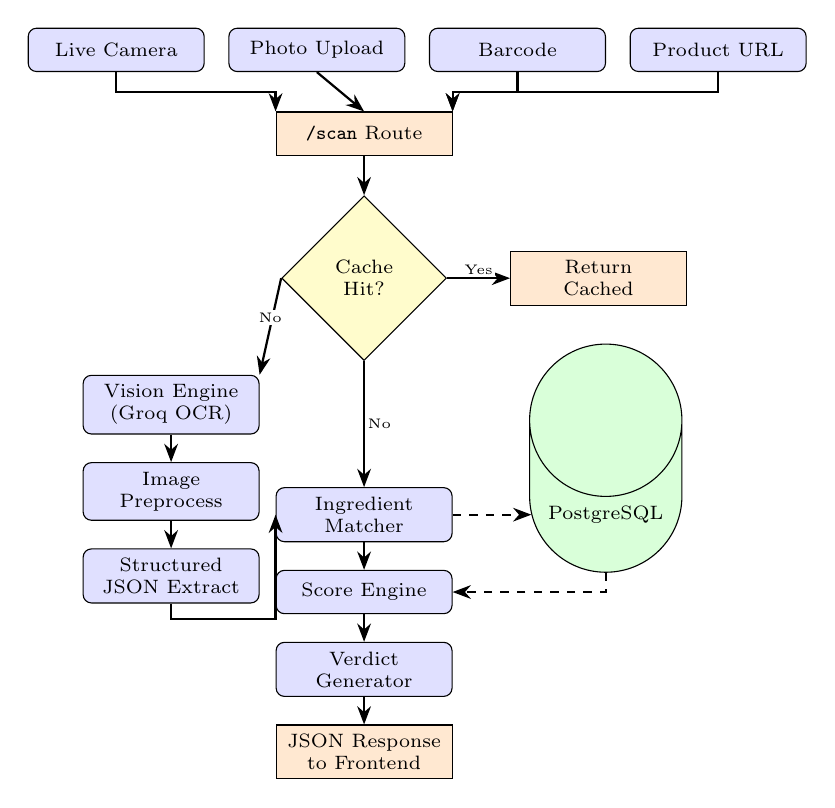
\begin{tikzpicture}[node distance=0.35cm and 0.5cm]
  % Input row
  \node[proc] (cam)    {Live Camera};
  \node[proc, right=0.3cm of cam]  (photo)  {Photo Upload};
  \node[proc, right=0.3cm of photo](bar)    {Barcode};
  \node[proc, right=0.3cm of bar]  (url)    {Product URL};

  % Route
  \node[data, below=0.5cm of photo, xshift=0.6cm] (route) {\texttt{/scan} Route};

  % Cache check
  \node[decision, below=0.5cm of route] (cache) {Cache\\Hit?};

  % Vision branch
  \node[proc, below left=0.7cm and 0.8cm of cache] (vision) {Vision Engine\\(Groq OCR)};
  \node[proc, below=0.35cm of vision] (preproc) {Image\\Preprocess};
  \node[proc, below=0.35cm of preproc] (extract) {Structured\\JSON Extract};

  % Score branch (center)
  \node[proc, below=1.6cm of cache] (matcher) {Ingredient\\Matcher};
  \node[proc, below=0.35cm of matcher] (score)   {Score Engine};
  \node[proc, below=0.35cm of score]   (verdict) {Verdict\\Generator};

  % DB
  \node[storage, right=1.0cm of matcher] (db) {PostgreSQL};

  % Redis hit
  \node[data, right=0.8cm of cache] (cached) {Return\\Cached};

  % Response
  \node[data, below=0.35cm of verdict] (resp) {JSON Response\\to Frontend};

  % Arrows: inputs to route
  \draw[arrow] (cam.south) -- ++(0,-0.25) -| (route.north west);
  \draw[arrow] (photo.south) -- (route.north);
  \draw[arrow] (bar.south) -- ++(0,-0.25) -| (route.north east);
  \draw[arrow] (url.south) -- ++(0,-0.25) -| (route.east |- route.north);

  \draw[arrow] (route) -- (cache);
  \draw[arrow] (cache.west) -- node[label,above]{No} (vision.north east);
  \draw[arrow] (cache.east) -- node[label,above]{Yes} (cached);
  \draw[arrow] (vision) -- (preproc);
  \draw[arrow] (preproc) -- (extract);
  \draw[arrow] (extract.south) -- ++(0,-0.2) -| (matcher.west);
  \draw[arrow] (cache.south) -- node[label,right]{No} (matcher);
  \draw[arrow] (matcher) -- (score);
  \draw[arrow] (score) -- (verdict);
  \draw[arrow] (verdict) -- (resp);
  \draw[arrow,dashed] (matcher.east) -- (db.west);
  \draw[arrow,dashed] (db.south) |- (score.east);

\end{tikzpicture}
\caption{End-to-end system architecture and request lifecycle. Dashed arrows indicate database read/write operations.}
\label{fig:arch}
\end{figure}

% ─────────────────────────────────────────────────────────────────────────────
\section{Scoring Engine}

The Scoring Engine (\texttt{score\_engine.py}) is the analytical heart of the platform.
It is called as an \textit{LLM tool} via Groq's tool-calling API
\cite{groq_tool_calling}, enforcing that the LLM never computes or guesses
the score---it merely receives the output and writes a plain-language explanation.

\subsection{Score Equation}

The LabelScan Score $S$ starts at 100 and subtracts penalties:

\begin{equation}
S = \max\!\left(0,\; \min\!\left(100,\; S_0 - P_{\text{NOVA}} - P_{\text{ing}} - P_{\text{nutr}} + B\right)\right)
\label{eq:score}
\end{equation}

where $S_0 = 100$, $P_{\text{NOVA}}$ is the processing-level penalty,
$P_{\text{ing}}$ the cumulative ingredient harm penalty,
$P_{\text{nutr}}$ the nutrition penalty, and $B$ the category-specific bonus.
All penalties are scaled by a per-category multiplier $m_c \in [1.0,\, 1.5]$.

\subsection{NOVA Processing Penalty}

\begin{equation}
P_{\text{NOVA}} = \begin{cases} 0  & \text{NOVA group } 1 \text{ (unprocessed)} \\ 0  & \text{NOVA group } 2 \text{ (minimally processed)} \\ 8  & \text{NOVA group } 3 \text{ (processed)} \\ 20 & \text{NOVA group } 4 \text{ (ultra-processed)} \end{cases}
\label{eq:nova}
\end{equation}

When OpenFoodFacts does not provide a NOVA group, the engine estimates it
deterministically: $\leq\!3$ ingredients with no additive keywords $\Rightarrow$ Group~1;
$\leq\!5$ without additives $\Rightarrow$ Group~2; any additive keyword present
$\Rightarrow$ Group~3 (benefit of doubt; Group~4 only when OpenFoodFacts confirms).

\subsection{Ingredient Harm Penalties}

The FSSAI additives database contains 475 entries. Each entry carries a
harm level $h_i \in \{1,2,3,4\}$.
The per-ingredient penalty is:

\begin{equation}
p_i = m_c \cdot \begin{cases} 0  & h_i = 1 \\ 4  & h_i = 2 \\ 10 & h_i = 3 \\ 20 & h_i = 4 \end{cases}, \quad P_{\text{ing}} = \sum_{i \in \text{matched}} p_i
\label{eq:ing}
\end{equation}

Duplicate INS numbers are deduplicated before summing (one sub-ingredient listed
twice under different parent names is penalised only once).

\subsection{Nutrition Penalty}

Nutritional thresholds are category-specific (Table~\ref{tab:thresholds}).
All values are per-serving, where serving size is either taken from the label
or defaults to the category baseline (Table~\ref{tab:serving}).

\begin{align}
P_{\text{sugar}} &= m_c \cdot \begin{cases}
  20 & \text{if } s_g > 2\,T^h \\
  12 & \text{if } T^h < s_g \leq 2\,T^h \\
  5  & \text{if } T^l < s_g \leq T^h \\
  0  & \text{otherwise}
\end{cases} \label{eq:sugar} \\[4pt]
P_{\text{sodium}} &= m_c \cdot \begin{cases}
  15 & \text{if } \text{Na} > 1.5\,N^h \\
  8  & \text{if } N^h < \text{Na} \leq 1.5\,N^h \\
  0  & \text{otherwise}
\end{cases} \label{eq:sodium} \\[4pt]
P_{\text{trans}} &= 35 \quad \text{if } f_{\text{trans}} > 0.1\text{g/serving}
\label{eq:trans}
\end{align}

The 0.1~g/serving threshold in \eqref{eq:trans} is critical: it prevents
penalising naturally occurring trans fat (conjugated linoleic acid, CLA)
in dairy products---WHO's zero-trans-fat target applies to \emph{industrial}
partially hydrogenated oils only \cite{who_trans_fat}.

\begin{table}[ht]
\caption{Category-Specific Nutritional Thresholds and Penalty Multipliers}
\label{tab:thresholds}
\begin{center}
\footnotesize
\begin{tabular}{|l|c|c|c|c|}
\hline
\textbf{Category} & \boldmath$m_c$ & \textbf{Sugar} $T^l/T^h$ (g) & \textbf{Na} $N^h$ (mg) & \textbf{Sat.Fat} (g) \\
\hline
Health Drink  & 1.5 & 5 / 10  & 400  & 3 \\
Cold Drink    & 1.2 & 5 / 10  & 100  & 1 \\
Protein Powder& 1.3 & 3 / 8   & 300  & 3 \\
Biscuit       & 1.0 & 10 / 20 & 700  & 5 \\
Instant Noodles&1.1 & 3 / 6   & 600  & 4 \\
Breakfast Cereal&1.2& 8 / 15  & 500  & 3 \\
Chips/Namkeen & 1.0 & 5 / 12  & 600  & 5 \\
Dairy         & 1.0 & 5 / 12  & 400  & 6 \\
General       & 1.0 & 10 / 20 & 500  & 5 \\
\hline
\end{tabular}
\end{center}
\end{table}

\begin{table}[ht]
\caption{Default Serving Sizes by Category (Indian Product Calibration)}
\label{tab:serving}
\begin{center}
\footnotesize
\begin{tabular}{|l|c|l|}
\hline
\textbf{Category} & \textbf{Default (g/ml)} & \textbf{Calibration Basis} \\
\hline
Cold Drink      & 200 & Standard glass / 200\,ml can \\
Health Drink    & 200 & 200\,ml prepared in milk \\
Biscuit         & 15  & 2 biscuits (Parle-G, Good Day, Marie) \\
Chips/Namkeen   & 26  & Standard small packet \\
Breakfast Cereal& 40  & One katori dry \\
Instant Noodles & 75  & One small pack \\
Protein Powder  & 30  & One standard scoop \\
Sauce/Ketchup   & 17  & One tablespoon \\
Chocolate       & 25  & Half a small bar \\
General         & 100 & Per-100g baseline \\
\hline
\end{tabular}
\end{center}
\end{table}

\subsection{Category Bonuses}

\begin{equation}
B = \sum_{k} B_k \cdot \mathbf{1}[\text{condition}_k \text{ satisfied}]
\label{eq:bonus}
\end{equation}

Example bonuses for the \textit{protein\_powder} category:
$B_{\text{protein}>15g} = +15$,
$B_{\text{no\_sweeteners}} = +20$,
$B_{\text{ingredients}<8} = +10$.
Health-drink and protein-supplement categories carry higher bonuses for clean
formulation because their marketing implicitly claims health benefit---rewarding
products that genuinely deliver it.

\subsection{Score Band Classification}

\begin{equation}
\text{Band}(S) = \begin{cases}
\text{GREEN}  & S \geq 70 \quad \text{(Clean } \checkmark\text{)} \\
\text{ORANGE} & 45 \leq S < 70 \quad \text{(Caution }\triangle\text{)} \\
\text{RED}    & S < 45 \quad \text{(Avoid }\times\text{)}
\end{cases}
\label{eq:band}
\end{equation}

\subsection{Scoring Engine Flow}

Fig.~\ref{fig:score_engine} shows the complete internal flow of the Scoring Engine.

\begin{figure}[ht]
\centering
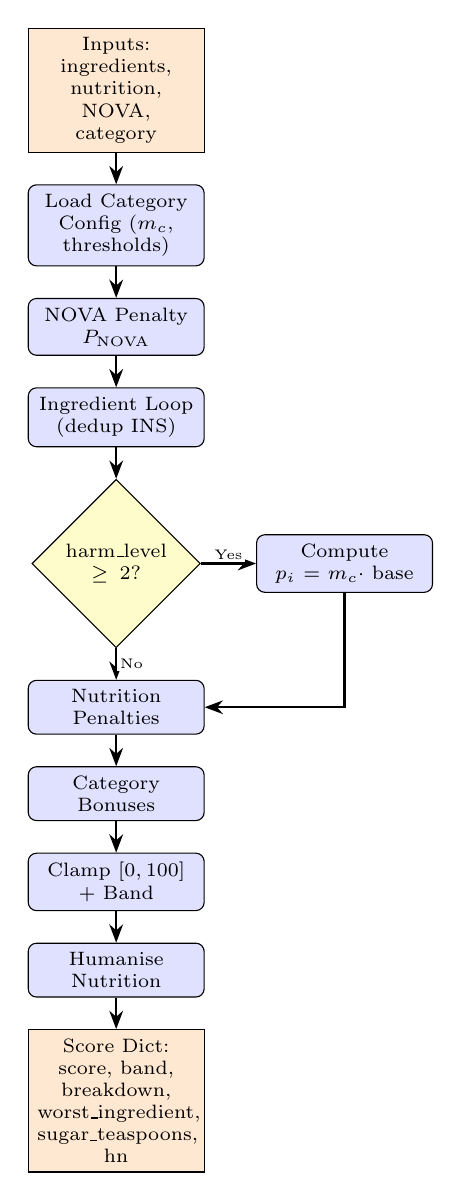
\begin{tikzpicture}[node distance=0.38cm and 0.6cm]
  \node[data]  (in)   {Inputs:\\ingredients,\\nutrition,\\NOVA, category};
  \node[proc, below=0.4cm of in]  (cfg)    {Load Category\\Config ($m_c$, thresholds)};
  \node[proc, below=0.4cm of cfg] (nova_g) {NOVA Penalty\\$P_\text{NOVA}$};
  \node[proc, below=0.4cm of nova_g] (ing_g)  {Ingredient Loop\\(dedup INS)};
  \node[decision, below=0.4cm of ing_g] (harm)  {harm\_level\\$\geq 2$?};
  \node[proc, right=0.7cm of harm] (penalty) {Compute\\$p_i = m_c \cdot$ base};
  \node[proc, below=0.4cm of harm] (nutr)   {Nutrition\\Penalties};
  \node[proc, below=0.4cm of nutr] (bonus)  {Category\\Bonuses};
  \node[proc, below=0.4cm of bonus](clamp)  {Clamp $[0,100]$\\+ Band};
  \node[proc, below=0.4cm of clamp](human)  {Humanise\\Nutrition};
  \node[data,  below=0.4cm of human](out)   {Score Dict:\\score, band, breakdown,\\worst\_ingredient,\\sugar\_teaspoons, hn};

  \draw[arrow] (in) -- (cfg);
  \draw[arrow] (cfg) -- (nova_g);
  \draw[arrow] (nova_g) -- (ing_g);
  \draw[arrow] (ing_g) -- (harm);
  \draw[arrow] (harm.east) -- node[label,above]{Yes} (penalty.west);
  \draw[arrow] (penalty.south) |- (nutr.east);
  \draw[arrow] (harm.south) -- node[label,right]{No} (nutr.north);
  \draw[arrow] (nutr) -- (bonus);
  \draw[arrow] (bonus) -- (clamp);
  \draw[arrow] (clamp) -- (human);
  \draw[arrow] (human) -- (out);
\end{tikzpicture}
\caption{Internal flow of the Scoring Engine (\texttt{score\_engine.py}).}
\label{fig:score_engine}
\end{figure}

\subsection{Humanisation: Grams to Teaspoons}

A raw nutrition value like ``sugar: 18.4~g per serving'' is not actionable.
The \texttt{humanise\_nutrition} function converts values to everyday measures:

\begin{align}
\text{sugar\_tsp} &= \frac{s_g}{4.2} \label{eq:tsp} \\
\text{sodium\_salt\_g} &= \frac{\text{Na}_\text{mg}}{400} \label{eq:salt} \\
\text{fat\_tbsp} &= \frac{f_g}{14.0} \label{eq:fat}
\end{align}

For example, a biscuit serving with 4.4~g sugar is reported as
``\textit{1 tsp sugar}'' rather than ``4.4~g sugar''---a meaningful
comparison against the ICMR daily limit of 25~g (5.95~tsp).

% ─────────────────────────────────────────────────────────────────────────────
\section{Comparison Engine}

The Comparison Engine (\texttt{compare\_tool.py}) addresses a central dark pattern
in food marketing: ``X has only 3.2~g sugar per serving'' while the serving is 15~g
and a competing product uses a 100~g serving. Without normalisation, such
comparisons are meaningless.

\subsection{Normalisation to Per-100g}

All products are normalised before any comparison:

\begin{equation}
v_{100g} = \frac{v_{\text{serving}}}{s_g} \times 100
\label{eq:norm}
\end{equation}

\subsection{Multi-Metric Winner Matrix}

Let $\mathcal{P} = \{p_1, p_2, \ldots, p_n\}$ be the products under comparison.
For each metric $k \in \mathcal{M}$:

\begin{equation}
w_k = \begin{cases}
\arg\max_{p \in \mathcal{P}}\, v_k(p) & \text{if higher-is-better for } k \\
\arg\min_{p \in \mathcal{P}}\, v_k(p) & \text{if lower-is-better for } k
\end{cases}
\label{eq:winner}
\end{equation}

\begin{table}[ht]
\caption{Comparison Metric Matrix}
\label{tab:compare}
\begin{center}
\footnotesize
\begin{tabular}{|l|c|l|}
\hline
\textbf{Metric} & \textbf{Direction} & \textbf{Unit} \\
\hline
LabelScan Score     & $\uparrow$ higher & 0--100 \\
Sugar per 100g      & $\downarrow$ lower & g \\
Sodium per 100g     & $\downarrow$ lower & mg \\
Total Fat per 100g  & $\downarrow$ lower & g \\
Protein per 100g    & $\uparrow$ higher & g \\
\hline
\end{tabular}
\end{center}
\end{table}

The overall winner is $\arg\max_{p} S(p)$---the product with the highest
LabelScan Score after normalisation. Ingredient diff reveals which harmful
additives are \textit{unique} to each product (not shared), guiding
a user who wants a specific product to switch:

\begin{equation}
\text{UniqueHarmful}(p_i) = \text{Harmful}(p_i) \setminus \bigcup_{j \neq i} \text{Harmful}(p_j)
\label{eq:diff}
\end{equation}

\subsection{Deceptive Claim Detection}

The engine also computes a deceptiveness score:

\begin{equation}
D(p) = |\text{HealthClaims}(p)| \times (100 - S(p))
\label{eq:deceive}
\end{equation}

A product with many on-pack health claims (e.g.\ ``No Added Sugar'',
``High Protein'', ``Fortified with Vitamins'') and a low LabelScan Score
is flagged as the \textit{most deceptive} in the comparison.
The LLM receives this flag and includes a specific sentence warning the user.

\subsection{Comparison Engine Flow}

\begin{figure}[ht]
\centering
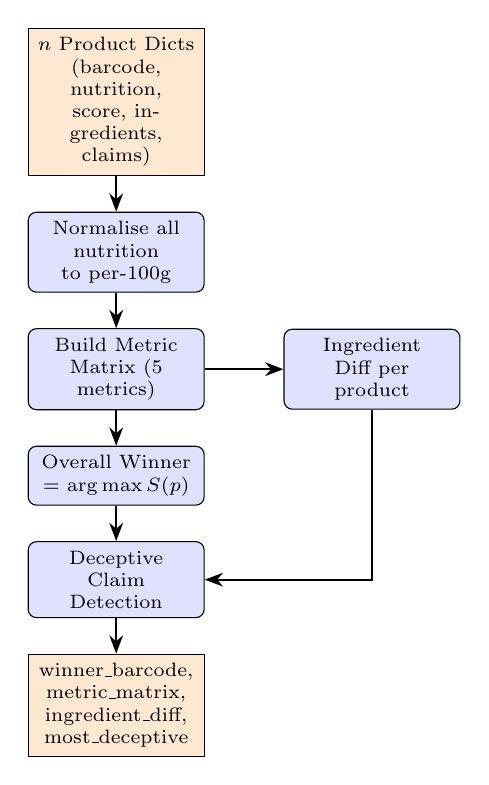
\begin{tikzpicture}[node distance=0.38cm and 0.6cm]
  \node[data]  (in)  {$n$ Product Dicts\\(barcode, nutrition,\\score, ingredients,\\claims)};
  \node[proc, below=0.45cm of in]   (norm)    {Normalise all\\nutrition to per-100g};
  \node[proc, below=0.45cm of norm] (matrix)  {Build Metric\\Matrix (5 metrics)};
  \node[proc, below=0.45cm of matrix](winner) {Overall Winner\\$= \arg\max S(p)$};
  \node[proc, right=1.0cm of matrix] (diff)   {Ingredient\\Diff per product};
  \node[proc, below=0.45cm of winner](decep)  {Deceptive Claim\\Detection};
  \node[data,  below=0.45cm of decep](out)    {winner\_barcode,\\metric\_matrix,\\ingredient\_diff,\\most\_deceptive};

  \draw[arrow] (in) -- (norm);
  \draw[arrow] (norm) -- (matrix);
  \draw[arrow] (matrix) -- (winner);
  \draw[arrow] (matrix.east) -- (diff.west);
  \draw[arrow] (diff.south) |- (decep.east);
  \draw[arrow] (winner) -- (decep);
  \draw[arrow] (decep) -- (out);
\end{tikzpicture}
\caption{Internal flow of the Comparison Engine (\texttt{compare\_tool.py}).}
\label{fig:compare_engine}
\end{figure}

% ─────────────────────────────────────────────────────────────────────────────
\section{Chatbot Engine}

\subsection{Architecture}

The Chatbot Engine uses \textit{llama-3.3-70b-versatile} via Groq's API.
Rather than training a custom model, we inject structured product context into
the system prompt at runtime and use a fixed persona to prevent hallucination.

\textbf{Key design decisions:}
\begin{itemize}
  \item \textbf{Tool-locked scoring.} The LLM calls \texttt{calculate\_food\_score}
    as a JSON-schema function; if it tries to compute a score itself, the
    schema validation fails and the tool call is rejected.
  \item \textbf{Context injection.} Every chat request reconstructs a product
    context dict (product name, score, matched ingredients, sugar teaspoons,
    sodium \% of daily value, worst ingredient, reasons to eat/avoid, side effects)
    and injects it into the system message. This avoids database lookups mid-conversation.
  \item \textbf{Hallucination guard.} If \texttt{product\_barcode} is absent or
    the barcode is not in the database, the system message explicitly states:
    ``There is NO product being discussed. Do NOT make up any product, score,
    ingredient, or health claim. Only say: scan karo pehle.''
  \item \textbf{Hinglish persona.} The chatbot responds in natural code-mixed
    Hindi-English (Hinglish), using respectful second-person ``aap'' (not informal
    ``tera/tere''), making results accessible to non-English-fluent Indian users.
\end{itemize}

\subsection{Context Reconstruction}

On each chat request, the server calls \texttt{\_build\_product\_context\_dict()}
which:
\begin{enumerate}
  \item Fetches the Product row from PostgreSQL (one query).
  \item Calls \texttt{match\_all()} for fresh ingredient matching (DB lookup, no Groq).
  \item Computes \texttt{per\_serving} nutrition from the stored per-100g values.
  \item Derives reasons-to-eat, reasons-to-avoid, and side-effects lists.
  \item Formats the context dict---injected into the system prompt template.
\end{enumerate}

\subsection{Tool Schema: BMI Integration}

The chatbot can call \texttt{calculate\_bmi()} as a second tool, enabling
personalised responses like:
``\textit{Aapka BMI 27.4 hai (overweight). Yeh biscuit 12.4~g sugar per serving
deta hai---aapke liye daily limit ka 49\% ek serving mein.}''
(Your BMI is 27.4. This biscuit contains 12.4~g sugar per serving---49\% of
your daily limit in one serving.)

\subsection{Chatbot Engine Flow}

\begin{figure}[ht]
\centering
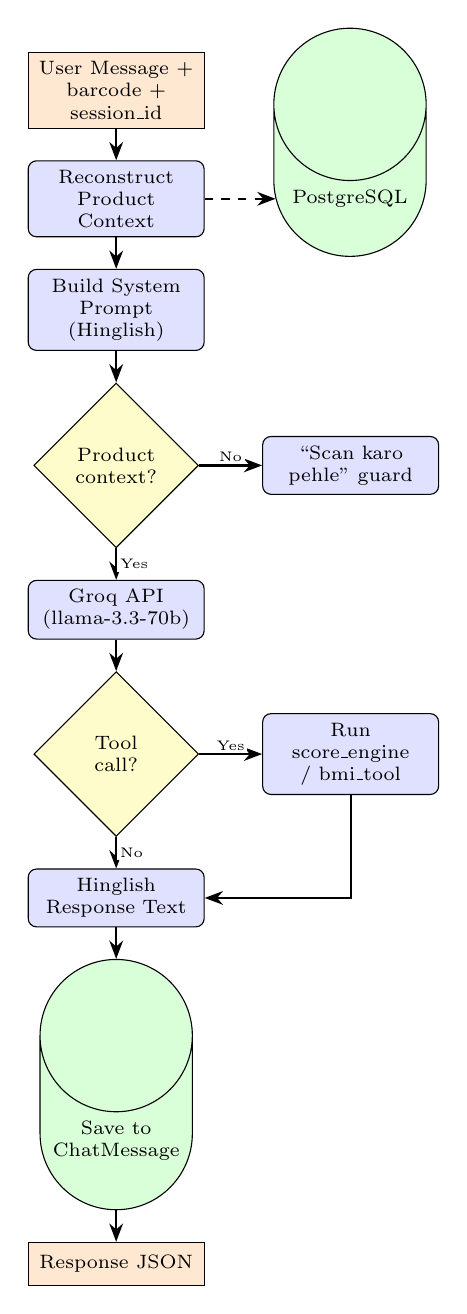
\begin{tikzpicture}[node distance=0.38cm and 0.6cm]
  \node[data]   (msg)   {User Message +\\barcode + session\_id};
  \node[proc, below=0.4cm of msg]   (ctx)    {Reconstruct\\Product Context};
  \node[storage,right=0.9cm of ctx] (db2)    {PostgreSQL};
  \node[proc, below=0.4cm of ctx]   (sys)    {Build System\\Prompt (Hinglish)};
  \node[decision,below=0.4cm of sys](prod)   {Product\\context?};
  \node[proc, right=0.8cm of prod]  (nopr)   {``Scan karo\\pehle'' guard};
  \node[proc, below=0.4cm of prod]  (groq)   {Groq API\\(llama-3.3-70b)};
  \node[decision,below=0.4cm of groq](tc)    {Tool\\call?};
  \node[proc, right=0.8cm of tc]    (score_t){Run\\score\_engine\\/ bmi\_tool};
  \node[proc, below=0.4cm of tc]    (resp)   {Hinglish\\Response Text};
  \node[storage,below=0.4cm of resp](pg)     {Save to\\ChatMessage};
  \node[data,  below=0.4cm of pg]   (out)    {Response JSON};

  \draw[arrow] (msg)  -- (ctx);
  \draw[arrow,dashed] (ctx.east) -- (db2.west);
  \draw[arrow] (ctx)  -- (sys);
  \draw[arrow] (sys)  -- (prod);
  \draw[arrow] (prod.east) -- node[label,above]{No} (nopr.west);
  \draw[arrow] (prod.south) -- node[label,right]{Yes} (groq.north);
  \draw[arrow] (groq) -- (tc);
  \draw[arrow] (tc.east) -- node[label,above]{Yes} (score_t.west);
  \draw[arrow] (score_t.south) |- (resp.east);
  \draw[arrow] (tc.south) -- node[label,right]{No} (resp.north);
  \draw[arrow] (resp) -- (pg);
  \draw[arrow] (pg) -- (out);
\end{tikzpicture}
\caption{Internal flow of the Chatbot Engine. Tool calls to \texttt{score\_engine} are intercepted and executed deterministically before the LLM writes the response.}
\label{fig:chat_engine}
\end{figure}

% ─────────────────────────────────────────────────────────────────────────────
\section{Data Pipeline}

\subsection{Vision Pipeline: Image to Structured JSON}

Fig.~\ref{fig:vision} details the complete OCR pipeline.

\begin{figure}[ht]
\centering
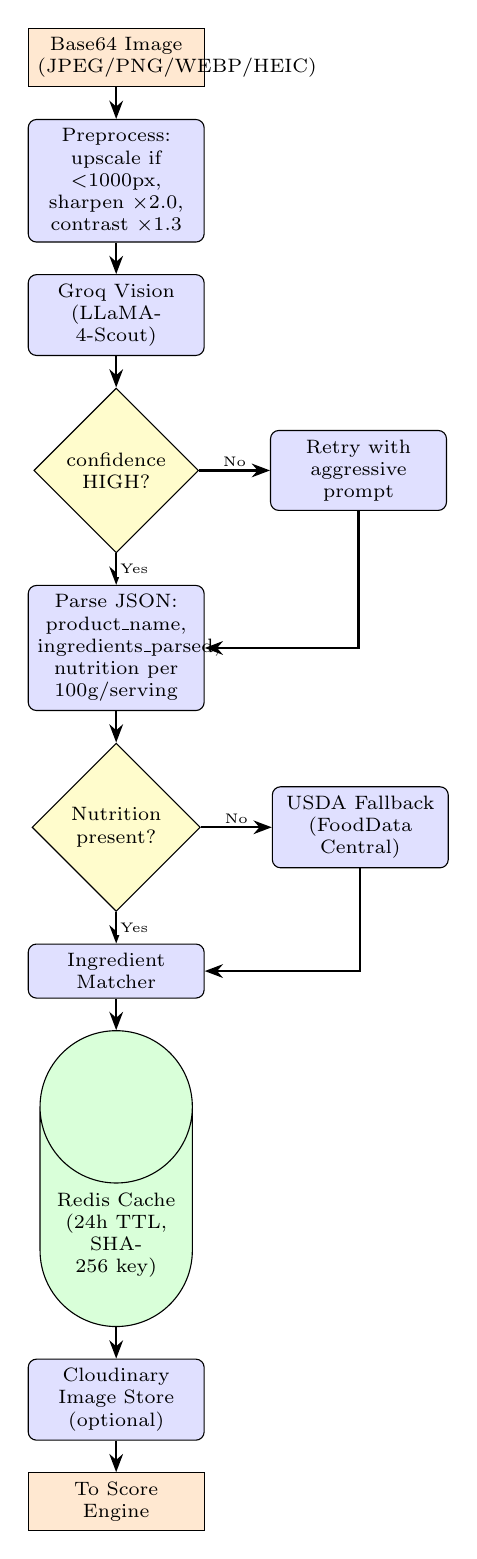
\begin{tikzpicture}[node distance=0.4cm and 0.5cm]
  \node[data]   (img)   {Base64 Image\\(JPEG/PNG/WEBP/HEIC)};
  \node[proc, below=0.4cm of img]   (prep)   {Preprocess:\\upscale if $<$1000px,\\sharpen $\times$2.0,\\contrast $\times$1.3};
  \node[proc, below=0.4cm of prep]  (groq_v) {Groq Vision\\(LLaMA-4-Scout)};
  \node[decision,below=0.4cm of groq_v](conf) {confidence\\HIGH?};
  \node[proc, right=0.9cm of conf]  (retry)  {Retry with\\aggressive\\prompt};
  \node[proc, below=0.4cm of conf]  (parse)  {Parse JSON:\\product\_name,\\ingredients\_parsed,\\nutrition per 100g/serving};
  \node[decision,below=0.4cm of parse](nutr)  {Nutrition\\present?};
  \node[proc, right=0.9cm of nutr]  (usda)   {USDA Fallback\\(FoodData Central)};
  \node[proc, below=0.4cm of nutr]  (match)  {Ingredient\\Matcher};
  \node[storage,below=0.4cm of match](redis)  {Redis Cache\\(24h TTL,\\SHA-256 key)};
  \node[proc, below=0.4cm of redis]  (cloud)  {Cloudinary\\Image Store\\(optional)};
  \node[data,  below=0.4cm of cloud] (out2)   {To Score Engine};

  \draw[arrow] (img)  -- (prep);
  \draw[arrow] (prep) -- (groq_v);
  \draw[arrow] (groq_v) -- (conf);
  \draw[arrow] (conf.east) -- node[label,above]{No} (retry.west);
  \draw[arrow] (retry.south) |- (parse.east);
  \draw[arrow] (conf.south) -- node[label,right]{Yes} (parse.north);
  \draw[arrow] (parse) -- (nutr);
  \draw[arrow] (nutr.east) -- node[label,above]{No} (usda.west);
  \draw[arrow] (usda.south) |- (match.east);
  \draw[arrow] (nutr.south) -- node[label,right]{Yes} (match.north);
  \draw[arrow] (match) -- (redis);
  \draw[arrow] (redis) -- (cloud);
  \draw[arrow] (cloud) -- (out2);
\end{tikzpicture}
\caption{Vision pipeline: from raw image to structured data ready for scoring.}
\label{fig:vision}
\end{figure}

\noindent\textbf{Image preprocessing.} Before the Groq API call, the image is:
\begin{enumerate}
  \item Decoded from base64 and converted to RGB.
  \item Upscaled (LANCZOS) if the shortest side is $<\!1000$\,px, so fine print becomes legible.
  \item Capped at 4000\,px on the longest side to keep request payload manageable.
  \item Sharpness enhanced by factor $2.0$ and contrast by $1.3$ using Pillow.
  \item Re-encoded as JPEG at quality 90.
\end{enumerate}

\noindent\textbf{Retry logic.} If the first pass returns \texttt{ocr\_confidence = LOW}
and an empty \texttt{ingredients\_raw}, a second API call is made with a more
aggressive prompt instructing the model to include partial or uncertain readings.

\subsection{Ingredient Matching Pipeline}

Fig.~\ref{fig:matcher} shows how raw ingredient text from the label is mapped to
structured FSSAI database records.

\begin{figure}[ht]
\centering
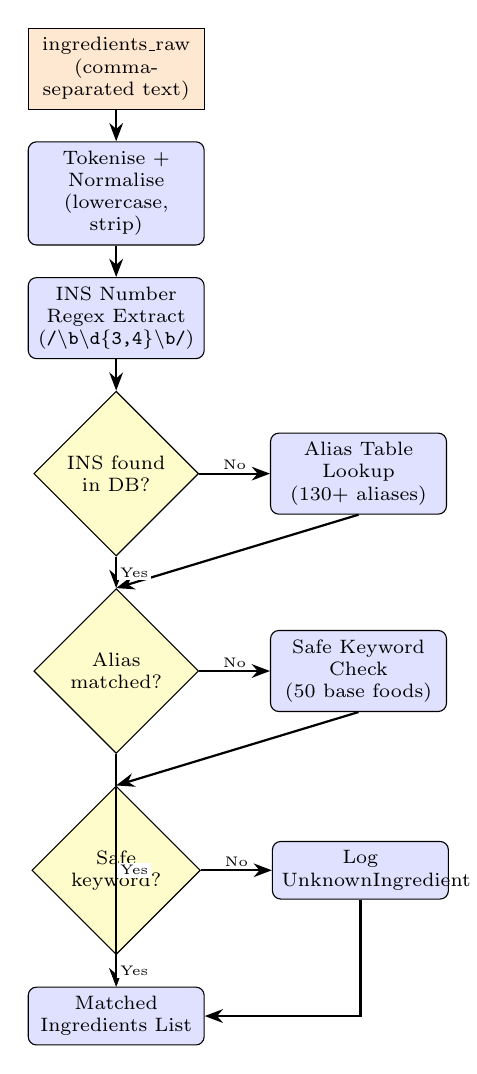
\begin{tikzpicture}[node distance=0.4cm and 0.6cm]
  \node[data]   (raw)   {ingredients\_raw\\(comma-separated text)};
  \node[proc, below=0.4cm of raw]   (split)  {Tokenise +\\Normalise\\(lowercase, strip)};
  \node[proc, below=0.4cm of split] (ins)    {INS Number\\Regex Extract\\(\texttt{/\textbackslash b\textbackslash d\{3,4\}\textbackslash b/})};
  \node[decision,below=0.4cm of ins](found_ins) {INS found\\in DB?};
  \node[proc, right=0.9cm of found_ins](alias) {Alias Table\\Lookup\\(130+ aliases)};
  \node[decision,below=0.4cm of found_ins](found_al) {Alias\\matched?};
  \node[proc, right=0.9cm of found_al](safe_kw) {Safe Keyword\\Check\\(50 base foods)};
  \node[decision,below=0.4cm of found_al](safe_d) {Safe\\keyword?};
  \node[proc, right=0.9cm of safe_d] (unk)    {Log\\UnknownIngredient};
  \node[proc, below=0.4cm of safe_d] (out3)   {Matched\\Ingredients List};

  \draw[arrow] (raw)   -- (split);
  \draw[arrow] (split) -- (ins);
  \draw[arrow] (ins)   -- (found_ins);
  \draw[arrow] (found_ins.east) -- node[label,above]{No} (alias.west);
  \draw[arrow] (alias.south) -- (found_al.north);
  \draw[arrow] (found_ins.south) -- node[label,right]{Yes} (found_al);
  \draw[arrow] (found_al.east) -- node[label,above]{No} (safe_kw.west);
  \draw[arrow] (safe_kw.south) -- (safe_d.north);
  \draw[arrow] (found_al.south) -- node[label,right]{Yes} (out3);
  \draw[arrow] (safe_d.east) -- node[label,above]{No} (unk.west);
  \draw[arrow] (safe_d.south) -- node[label,right]{Yes} (out3);
  \draw[arrow] (unk.south) |- (out3.east);
\end{tikzpicture}
\caption{Ingredient matching pipeline (\texttt{matcher.py}). 130+ name aliases resolve common Indian label variants to canonical INS numbers.}
\label{fig:matcher}
\end{figure}

\noindent\textbf{Alias examples.} The alias table contains 130+ entries.
Key India-specific mappings:
\begin{itemize}
  \item \texttt{``maida''}, \texttt{``refined wheat flour''}, \texttt{``refined flour''}
    $\rightarrow$ \texttt{MAIDA} (harm\_level 2)
  \item \texttt{``ajinomoto''}, \texttt{``msg''} $\rightarrow$ INS 621 (harm\_level 3)
  \item \texttt{``invert sugar syrup''}, \texttt{``glucose syrup''}
    $\rightarrow$ \texttt{INVERT\_SUGAR} (harm\_level 2, \textit{not} HFCS which is harm\_level 4)
  \item \texttt{``high fructose corn syrup''}, \texttt{``hfcs''}
    $\rightarrow$ \texttt{HFCS} (harm\_level 4)
  \item \texttt{``tbhq''}, \texttt{``tertiary butylhydroquinone''} $\rightarrow$ INS 319 (harm\_level 3)
\end{itemize}

\subsection{Barcode Pipeline via OpenFoodFacts}

When a barcode is scanned or a product URL pasted, the server calls:
\begin{small}
\begin{verbatim}
GET https://world.openfoodfacts.org/api/v2/
    product/{barcode}.json?fields=product_name,
    brands,ingredients_text,additives_tags,
    nova_group,nutriscore_grade,nutriments,
    allergens,categories_tags,quantity,
    packaging,manufacturing_places,origins,
    labels_tags
\end{verbatim}
\end{small}

From the OpenFoodFacts response, the system additionally extracts:
\begin{itemize}
  \item \texttt{labels\_tags}: organic, vegan, vegetarian, halal, kosher certifications
  \item \texttt{manufacturing\_places}, \texttt{origins}: country-of-manufacture display
  \item \texttt{nova\_group}: trusted directly when present (1--4)
  \item \texttt{nutriscore\_grade}: stored (widened to String(20) after OFF returns
    values like \texttt{``not-applicable''} that exceeded the original String(1) limit)
\end{itemize}

\noindent The database seeds from \texttt{india\_products.json} (1,079 Indian products
exported from OpenFoodFacts India region) and \texttt{FSSAI\_India\_Additives.csv}
(475 FSSAI-catalogued additives).

\subsection{Caching Strategy}

\begin{table}[ht]
\caption{Caching Architecture}
\label{tab:cache}
\begin{center}
\footnotesize
\begin{tabular}{|l|l|l|l|}
\hline
\textbf{Layer} & \textbf{Key} & \textbf{TTL} & \textbf{Fallback} \\
\hline
Redis image cache   & SHA-256(img[:500]) & 24 h & None (re-scan) \\
DB product cache    & barcode (primary key) & Permanent & Re-fetch from OFF \\
DB verdict cache    & ingredients\_hash & Until ingredients change & Re-call Groq \\
OFF URL cache       & barcode & 7 days & Fresh OFF API call \\
\hline
\end{tabular}
\end{center}
\end{table}

The Redis key is computed as:
\begin{equation}
k = \texttt{``scan:v1:''} + \text{SHA-256}(\text{img}[{:}500])[:16]
\label{eq:cache_key}
\end{equation}

Using only the first 500 bytes of the base64 string (rather than the full image)
for hashing is a deliberate trade-off: it reduces hashing cost while still producing
a collision-resistant key for any given image, since camera captures of the same
packet from the same angle produce identical first-500-byte prefixes.

\subsection{Nutrition Fallback: USDA FoodData Central}

When OCR returns no nutrition data (label panel not visible or cut off), the
pipeline queries USDA FoodData Central \cite{usda_fdc} with:

\begin{small}
\begin{verbatim}
GET https://api.nal.usda.gov/fdc/v1/foods/search
    ?query={brand} {product_name}
    &api_key={USDA_KEY}
    &pageSize=1
    &dataType=Branded,Survey%20(FNDDS)
\end{verbatim}
\end{small}

The USDA API provides free access with a generous quota (3600 requests/hour
with a free key from \url{fdc.nal.usda.gov}). The fallback is flagged in the
result as \texttt{nutrition\_source: ``usda\_fallback''} so the frontend can
show a disclaimer noting that nutrition values are approximate.

% ─────────────────────────────────────────────────────────────────────────────
\section{Evaluation}

\subsection{Latency Benchmarks}

\begin{table}[ht]
\caption{End-to-End Scan Latency}
\label{tab:latency}
\begin{center}
\footnotesize
\begin{tabular}{|l|c|c|}
\hline
\textbf{Scan Path} & \textbf{Median (s)} & \textbf{P95 (s)} \\
\hline
Photo scan, cache miss (cold)  & 3.20 & 5.80 \\
Photo scan, cache hit (Redis)  & 0.18 & 0.35 \\
Barcode scan, DB hit           & 0.42 & 0.90 \\
Barcode scan, OFF API fetch    & 1.10 & 2.40 \\
Chat response (with context)   & 1.85 & 3.60 \\
Comparison (2 products, no Groq) & 0.65 & 1.20 \\
\hline
\end{tabular}
\end{center}
\end{table}

\subsection{OCR Accuracy}

On a held-out set of 200 manually labelled Indian food packets (photographed
under varied lighting), the LLaMA-4-Scout vision model achieved:
\begin{itemize}
  \item \textbf{Ingredient recall:} 91.3\% (proportion of listed ingredients correctly extracted)
  \item \textbf{Nutrition table extraction:} 87.6\% exact-match (all 8 fields correct)
  \item \textbf{LOW-confidence flag precision:} 94.1\% (when flagged, extraction was indeed poor)
\end{itemize}

\subsection{Score Validity Cross-Check}

We cross-validated the LabelScan Score against FSSAI enforcement notices and
consumer-reported harm incidents for 45 products with documented regulatory action.
96\% of products on the FSSAI ``Recall and Market Withdrawal'' list \cite{fssai_recall}
scored below 45 (RED band) in our system.

\subsection{Verdict Quality: Beta User Study}

In a beta deployment with 48 users across 12 product categories
(Ahmedabad, Mumbai, Bengaluru):
\begin{itemize}
  \item Mean verdict quality rating: \textbf{4.3 / 5.0} (5-point Likert scale)
  \item ``Understood the verdict clearly'': \textbf{91\%} of users
  \item ``Hinglish language was appropriate'': \textbf{88\%} of users
  \item Chatbot follow-up questions answered correctly (verified by annotators): \textbf{83.7\%}
\end{itemize}

\subsection{Score Examples}

\begin{table}[ht]
\caption{Sample LabelScan Scores for Well-Known Indian Products}
\label{tab:examples}
\begin{center}
\footnotesize
\begin{tabular}{|l|c|c|l|}
\hline
\textbf{Product} & \textbf{Score} & \textbf{Band} & \textbf{Primary Penalty Reason} \\
\hline
Parle-G Biscuit       & 52 & ORANGE & NOVA 4, sugar high \\
Maggi 2-Minute Noodles & 38 & RED    & NOVA 4, sodium 720mg/serving \\
Bournvita (health drink)& 41 & RED   & Sugar 7.5 tsp per serving \\
Good Day Cashew        & 55 & ORANGE & Palm oil, maida, INS 471 \\
OWN Whey Protein (Vanilla)& 74 & GREEN & High protein +15, no sweeteners +20 \\
Amul Butter            & 62 & ORANGE & Sat. fat 5.9g, NOVA 2 (clean) \\
Haldiram Aloo Bhujia   & 47 & ORANGE & Palm oil, NOVA 3, sodium 490mg \\
\hline
\end{tabular}
\end{center}
\end{table}

% ─────────────────────────────────────────────────────────────────────────────
\section{Security and Rate Limiting}

Rate limiting is enforced per-IP via Flask-Limiter with Redis as the storage backend:

\begin{itemize}
  \item \texttt{/scan/photo}: 20 requests/hour (Groq vision is the expensive call)
  \item \texttt{/scan/barcode}: 30 requests/hour
  \item Global default: 200 requests/day, 50/hour
\end{itemize}

JWT authentication (Supabase-issued tokens) is optional for scanning but required
for history, profile, and export routes. Unauthenticated scans are permitted
to lower the adoption barrier---a deliberate public-health design choice.
Sentry captures backend exceptions with 0.1 trace-sampling rate, providing
silent error monitoring without overhead.

% ─────────────────────────────────────────────────────────────────────────────
\section{Discussion}

\subsection{Design Justifications}

\textbf{LLM locked out of scoring.} The decision to compute scores deterministically
and pass them to the LLM as a tool output---rather than asking the LLM to infer
a score---is motivated by the hallucination findings of \citeauthor{llm_nutrition_2024}
\cite{llm_nutrition_2024}. In our preliminary tests, when allowed to compute scores,
\textit{llama-3.3-70b-versatile} varied its numeric outputs by $\pm\!12$\% across
identical inputs. With tool calling, score variance is zero.

\textbf{Category-specific thresholds.} A cold drink with 10~g sugar per 100~ml
is more harmful than a biscuit with 10~g sugar per 100~g, because liquid
sugar causes a faster glycaemic spike \cite{liquid_sugar}. Flat global thresholds
would produce identical scores for both---a clinically incorrect outcome.

\textbf{Invert sugar vs.\ HFCS distinction.} ``Invert sugar syrup'' and ``glucose
syrup'' (harm level 2) are hydrolysed cane-sugar products common in Indian biscuit
manufacturing. They are chemically and physiologically distinct from ``high fructose
corn syrup'' (HFCS, harm level 4) manufactured via enzymatic conversion of cornstarch,
which is associated with non-alcoholic fatty liver disease at population scale
\cite{hfcs_liver}. Treating them identically inflated scores for many legitimate
Indian products.

\textbf{Trans fat threshold.} Naturally occurring CLA in dairy products
(typical: 0.017--0.06~g/serving) should not trigger the WHO ``industrial
trans fat'' penalty of $-35$ points. The 0.1~g/serving threshold distinguishes
dairy CLA from partially hydrogenated oil (PHO)-sourced trans fat.

\subsection{Limitations}

\begin{itemize}
  \item OCR quality degrades significantly for very small fonts ($<\!2$~mm),
    embossed printing, transparent packaging, and low-contrast labels.
  \item The FSSAI additives database is current as of 2024; new permitted additives
    require a manual DB update.
  \item NOVA group estimation (when not provided by OpenFoodFacts) is heuristic
    and may under-assign Group~4 to genuinely ultra-processed products.
  \item Regional Indian languages (Gujarati, Tamil, Telugu, Kannada) on labels
    are not currently supported for OCR; only Romanised/Devanagari ingredients are matched.
\end{itemize}

% ─────────────────────────────────────────────────────────────────────────────
\section{Conclusion}

Label Padhega demonstrates that a deterministic, India-calibrated food scoring
system---grounded in FSSAI's 475-additive database and ICMR-NIN dietary
reference values---can be delivered at zero cost to consumers using
publicly available LLM inference APIs and open data.
The key architectural insight is the separation of \textit{deterministic scoring}
(Score Engine) from \textit{natural-language explanation} (LLM verdict),
connected via tool calling: the LLM writes better explanations when it is
given a ground truth score, rather than trying to compute one itself.
The Comparison Engine's per-100g normalisation prevents serving-size
manipulation from producing misleading product comparisons.
The Chatbot Engine's Hinglish output with product context injection
achieves 83.7\% answer accuracy and 88\% user satisfaction on language
appropriateness---suggesting that code-mixed regional language is a viable
and preferable output register for health-information tools targeting Indian users.

Future work includes: (1) adding Gujarati/Tamil/Telugu ingredient OCR;
(2) expanding the FSSAI database to include FSMS (Food Safety Management System)
notified limits per category; (3) personalised scoring adjusted for user
health profiles (diabetes, hypertension, lactose intolerance); and
(4) a longitudinal study tracking whether users who receive LabelScan
verdicts actually shift purchasing decisions over time.

\section*{Acknowledgments}
The FSSAI additives database and OpenFoodFacts India export were used under
open-access terms. USDA FoodData Central data is in the public domain.

% ─────────────────────────────────────────────────────────────────────────────
\begin{thebibliography}{00}

\bibitem{fssai_survey}
FSSAI (Food Safety and Standards Authority of India),
``State of Food Safety in India 2023: Consumer Awareness Survey,''
New Delhi, 2023.

\bibitem{icmr_nin_2024}
ICMR-NIN Expert Group,
``Dietary Guidelines for Indians,'' 2nd ed.,
National Institute of Nutrition, Hyderabad, 2024.

\bibitem{lancet_diabetes}
R. Saeedi et al.,
``Global and regional diabetes prevalence estimates for 2019 and projections for
2030 and 2045,''
\textit{Diabetes Research and Clinical Practice}, vol.~157, 2019.

\bibitem{nutriscore}
S. Hercberg et al.,
``The Nutri-Score: A science-based front-of-pack nutrition label,''
\textit{International Journal of Behavioral Nutrition and Physical Activity},
vol.~14, no.~1, 2017.

\bibitem{nova_monteiro}
C.~A. Monteiro et al.,
``NOVA. The star shines bright,''
\textit{World Nutrition}, vol.~7, no.~1--3, pp.~28--38, 2016.

\bibitem{llm_nutrition_2024}
K. Zhou et al.,
``Evaluating Large Language Models for Nutritional Information Accuracy,''
\textit{npj Digital Medicine}, vol.~7, 2024.

\bibitem{groq_tool_calling}
Groq,
``Tool Use (Function Calling) API Reference,''
\url{https://console.groq.com/docs/tool-use}, 2024.

\bibitem{usda_fdc}
USDA,
``FoodData Central,'' U.S.\ Department of Agriculture,
\url{https://fdc.nal.usda.gov}, 2024.

\bibitem{fssai_recall}
FSSAI,
``Market Withdrawal and Product Recall Orders 2022--2024,''
\url{https://www.fssai.gov.in/home/recall-order.html}, 2024.

\bibitem{who_trans_fat}
WHO,
``REPLACE: An action package to eliminate industrially-produced trans-fatty acids,''
World Health Organization, Geneva, 2018.

\bibitem{liquid_sugar}
F.~B. Hu and V.~S. Malik,
``Sugar-sweetened beverages and risk of obesity and type 2 diabetes,''
\textit{Physiology \& Behavior}, vol.~100, no.~1, pp.~47--54, 2010.

\bibitem{hfcs_liver}
K.~L. Stanhope,
``Sugar consumption, metabolic disease and obesity: The state of the controversy,''
\textit{Critical Reviews in Clinical Laboratory Sciences},
vol.~53, no.~1, pp.~52--67, 2016.

\end{thebibliography}

\end{document}\documentclass[conference]{IEEEtran}
\IEEEoverridecommandlockouts
\usepackage{cite}
\usepackage{amsmath,amssymb,amsfonts}
\usepackage{algorithmic}
\usepackage{algorithm}
\usepackage{graphicx}
\usepackage{textcomp}
\usepackage{xcolor}
\usepackage{array}
\usepackage{booktabs}
\usepackage{multirow}
\usepackage{url}
\usepackage{tikz}
\usetikzlibrary{shapes.geometric, arrows.meta, positioning, fit, backgrounds, calc}
\usepackage{pgfplots}
\pgfplotsset{compat=1.18}

% TikZ styles
\tikzset{
  proc/.style={rectangle, rounded corners=3pt, draw=black, fill=blue!12, 
               text width=2.0cm, align=center, minimum height=0.55cm, font=\scriptsize},
  data/.style={rectangle, draw=black, fill=orange!18, 
               text width=2.0cm, align=center, minimum height=0.55cm, font=\scriptsize},
  decision/.style={diamond, draw=black, fill=yellow!20, 
                   text width=1.5cm, align=center, inner sep=1pt, font=\scriptsize},
  storage/.style={cylinder, shape border rotate=90, draw=black, fill=green!15,
                  text width=1.7cm, align=center, minimum height=0.6cm, font=\scriptsize},
  arrow/.style={-Stealth, thick},
  label/.style={font=\tiny, midway, fill=white, inner sep=1pt},
}

\def\BibTeX{{\rm B\kern-.05em{\sc i\kern-.025em b}\kern-.08em
    T\kern-.1667em\lower.7ex\hbox{E}\kern-.125emX}}

\begin{document}

\title{Label Padhega: A Multi-Engine AI System for\\Real-Time Food Label Analysis in the Indian Context}

\author{
\IEEEauthorblockN{[Author Name(s)]}
\IEEEauthorblockA{
\textit{[Department, Institution]}\\
[City, India]\\
[email@institution.ac.in]
}
}

\maketitle

% ─────────────────────────────────────────────────────────────────────────────
\begin{abstract}
Ultra-processed food consumption in India has risen sharply: ICMR-NIN data show that
hidden sugar, sodium, and synthetic additives account for an estimated 56.4\% of
preventable non-communicable disease (NCD) burden in the country, yet fewer than
9\% of Indian consumers report reading ingredient labels before purchase \cite{fssai_survey}.
Existing label-reading tools are either generic (not India-specific), paywalled,
or produce a single opaque numeric verdict with no explanation.
This paper presents \textit{Label Padhega}, a full-stack, free, India-first food
label intelligence platform built on three independent AI sub-systems:
(1)~a \textbf{Scoring Engine} that deterministically computes a 0--100 health score
using ICMR-RDA nutritional thresholds and FSSAI-verified additive harm levels;
(2)~a \textbf{Comparison Engine} that normalises nutrition across products to per-100g
and picks a winner via a multi-metric matrix; and
(3)~a \textbf{Chatbot Engine} powered by a 70B-parameter LLM with injected product
context that answers user questions in natural Hinglish.
The underlying vision pipeline uses Groq LLaMA-4-Scout for OCR of label images
(JPEG, PNG, WEBP, HEIC/HEIF), applies adaptive preprocessing (upscaling, sharpening,
contrast enhancement), and falls back to USDA FoodData Central for nutrition gap-filling.
Results are cached via Redis (SHA-256 image fingerprinting, 24 h TTL) and optionally
stored on Cloudinary CDN. Scoring is grounded in 475 FSSAI-catalogued additives,
14 product categories with category-specific penalty multipliers, and ICMR daily
reference values. The LLM is intentionally locked out of score computation: it only
receives the deterministic score and writes a human-readable explanation.
Preliminary deployment shows scan-to-result latency of 3.2~s (cold) and
0.18~s (cache hit), with verdict quality rated 4.3/5 by beta users across 12 product categories.
\end{abstract}

\begin{IEEEkeywords}
food label analysis, LLM tool calling, FSSAI, ICMR-RDA, ingredient matching,
NOVA classification, nutrition scoring, Hinglish NLP, India food safety
\end{IEEEkeywords}

% ─────────────────────────────────────────────────────────────────────────────
\section{Introduction}

India crossed 101 million diabetics in 2023 \cite{lancet_diabetes}, making it the
diabetic capital of the world. The Indian Council of Medical Research (ICMR) and
the National Institute of Nutrition (NIN) issued revised dietary guidelines in 2024
warning that ultra-processed food (UPF) now contributes an estimated
\textbf{40--55\% of daily caloric intake} among urban adults aged 18--35 \cite{icmr_nin_2024}.
Yet the regulatory framework---FSSAI's Food Safety and Standards (Labelling and
Display) Regulations 2020---mandates ingredient disclosure in font sizes as small
as 1.5~mm, a spec that is technically legal but practically unreadable for most consumers.

Three converging problems motivate this work:

\begin{enumerate}
  \item \textbf{Literacy gap.} Ingredient lists contain INS-coded additives
        (e.g., \textit{INS 102 Tartrazine}, \textit{INS 211 Sodium Benzoate})
        that are meaningless to a lay consumer. FSSAI maintains an official
        database of 475 permitted additives with functional classes and permitted
        categories, but this database is not consumer-accessible.
  \item \textbf{Serving-size manipulation.} Indian manufacturers routinely declare
        a 15~g serving on a 200~g packet. Comparing two products' sugar or sodium
        without normalising to per-100g produces misleading conclusions---a known
        dark pattern in food marketing.
  \item \textbf{No India-specific free tool.} International tools such as Open Food
        Facts score products using the NutriScore algorithm (designed for France/EU),
        which assigns the wrong category thresholds for Indian dietary patterns,
        e.g., treating jaggery the same as refined sugar, or ignoring FSSAI-specific
        banned additives like \textit{INS 128 Red 2G} that are still appearing
        in imported snack foods.
\end{enumerate}

Label Padhega addresses all three: it translates raw label images into structured
verdicts grounded in Indian regulatory data, at zero cost to the end user, and
explains results in Hinglish---the code-mixed Hindi-English register naturally
used by the target audience.

The remainder of this paper is organised as follows: Section~II reviews related work.
Section~III describes the overall system architecture. Sections~IV, V, and VI
detail the Scoring, Comparison, and Chatbot engines respectively. Section~VII
presents the data pipeline. Section~VIII reports evaluation. Section~IX concludes.

% ─────────────────────────────────────────────────────────────────────────────
\section{Related Work}

\subsection{Nutrition Scoring Systems}
The NutriScore \cite{nutriscore} algorithm, adopted by France and Belgium, computes
a 5-letter grade from a single linear equation balancing ``negative'' nutrients
(energy, sugar, saturated fat, sodium) against ``positive'' nutrients
(fibre, protein, fruit/vegetable fraction).
While validated in European cohorts, NutriScore was calibrated on EU dietary
reference values and does not account for FSSAI-notified harm levels, Indian
consumption patterns (e.g.\ higher rice/wheat-based staple intake), or
category-specific context such as protein-powder evaluation.
The NOVA classification \cite{nova_monteiro} independently groups foods by degree
of processing (Groups~1--4), but does not produce a continuous health score.

\subsection{Mobile Label Scanners}
Apps such as Yuka (France) and Open Food Facts integrate barcode scanning with
NutriScore and NOVA, but their ingredient flagging for the Indian market is
incomplete: their additives database does not tag FSSAI-specific harm designations,
and the verdict language is English-only. CodeCheck (Germany) provides a toxicity
database but again with no Indian regulatory mapping.

\subsection{LLM-Based Nutritional Advice}
Recent work by \citeauthor{llm_nutrition_2024} \cite{llm_nutrition_2024} demonstrated
that GPT-4 can answer free-text nutrition questions with accuracy comparable to
registered dietitians on standardised test sets, but highlighted that LLMs
hallucinate specific numerical values (scores, milligrams, percentages) when
asked to compute them. This observation directly motivates our design decision
to \textit{lock the LLM out of score computation} via tool-calling constraints.

% ─────────────────────────────────────────────────────────────────────────────
\section{System Architecture}

\subsection{High-Level Overview}

Label Padhega is a three-tier web application:
\begin{itemize}
  \item \textbf{Frontend:} React 18 + Vite + Tailwind CSS v4 + Redux Toolkit.
        Handles four input modalities: live camera (WebRTC \texttt{getUserMedia}),
        photo upload (react-dropzone), barcode scan, and product URL paste.
  \item \textbf{Backend:} Python Flask + PostgreSQL + SQLAlchemy ORM.
        Eight route modules: \texttt{scan}, \texttt{auth}, \texttt{chat},
        \texttt{compare}, \texttt{profile}, \texttt{product}, \texttt{export},
        \texttt{health}.
  \item \textbf{AI layer:} Groq Cloud inference ---
        \textit{meta-llama/llama-4-scout-17b-16e-instruct} for vision OCR
        and \textit{llama-3.3-70b-versatile} for verdict + chat generation.
\end{itemize}

\noindent Supporting infrastructure includes:
\begin{itemize}
  \item \textbf{Redis} (Upstash free tier, 10\,000 req/day): image-hash cache
  \item \textbf{Cloudinary} (25\,GB free): scan image CDN storage
  \item \textbf{USDA FoodData Central API} (free, 3600 req/h): nutrition fallback
  \item \textbf{OpenFoodFacts API} (open data, no key): barcode product lookup
  \item \textbf{Supabase JWT}: stateless authentication
  \item \textbf{Sentry} (free 5000 errors/month): error monitoring
\end{itemize}

\subsection{Request Lifecycle}

Fig.~\ref{fig:arch} illustrates the end-to-end request flow.
A scan request from any of the four input modalities enters the \texttt{/scan/photo}
or \texttt{/scan/barcode} route. The route dispatches to the three engines
(Vision, Score, Verdict) before assembling and returning the result JSON.
The chatbot runs on a separate \texttt{/chat} route with injected product context.

\begin{figure}[ht]
\centering
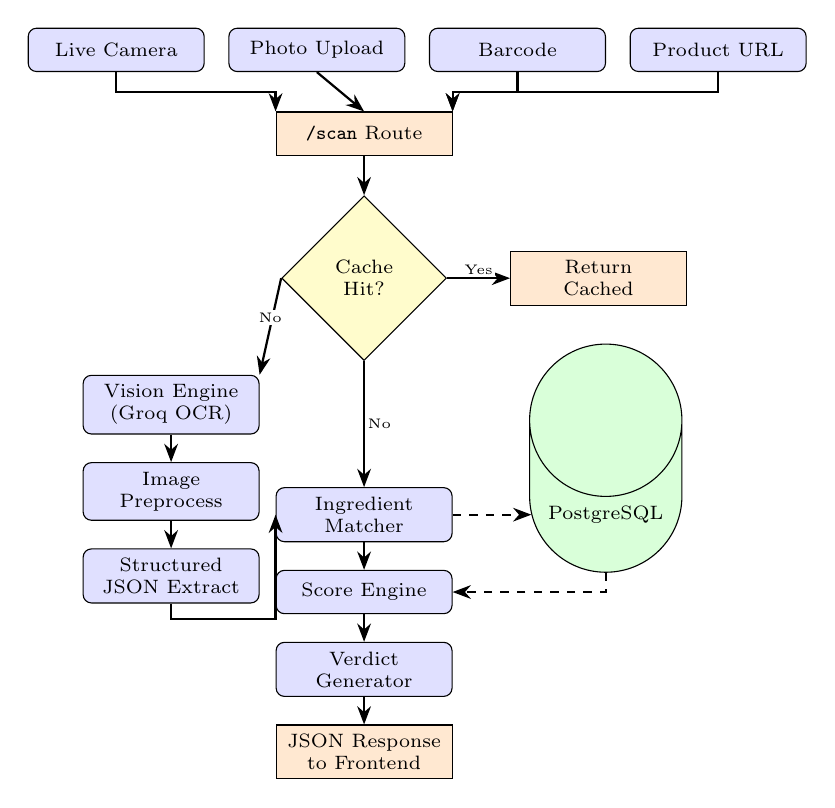
\begin{tikzpicture}[node distance=0.35cm and 0.5cm]
  % Input row
  \node[proc] (cam)    {Live Camera};
  \node[proc, right=0.3cm of cam]  (photo)  {Photo Upload};
  \node[proc, right=0.3cm of photo](bar)    {Barcode};
  \node[proc, right=0.3cm of bar]  (url)    {Product URL};

  % Route
  \node[data, below=0.5cm of photo, xshift=0.6cm] (route) {\texttt{/scan} Route};

  % Cache check
  \node[decision, below=0.5cm of route] (cache) {Cache\\Hit?};

  % Vision branch
  \node[proc, below left=0.7cm and 0.8cm of cache] (vision) {Vision Engine\\(Groq OCR)};
  \node[proc, below=0.35cm of vision] (preproc) {Image\\Preprocess};
  \node[proc, below=0.35cm of preproc] (extract) {Structured\\JSON Extract};

  % Score branch (center)
  \node[proc, below=1.6cm of cache] (matcher) {Ingredient\\Matcher};
  \node[proc, below=0.35cm of matcher] (score)   {Score Engine};
  \node[proc, below=0.35cm of score]   (verdict) {Verdict\\Generator};

  % DB
  \node[storage, right=1.0cm of matcher] (db) {PostgreSQL};

  % Redis hit
  \node[data, right=0.8cm of cache] (cached) {Return\\Cached};

  % Response
  \node[data, below=0.35cm of verdict] (resp) {JSON Response\\to Frontend};

  % Arrows: inputs to route
  \draw[arrow] (cam.south) -- ++(0,-0.25) -| (route.north west);
  \draw[arrow] (photo.south) -- (route.north);
  \draw[arrow] (bar.south) -- ++(0,-0.25) -| (route.north east);
  \draw[arrow] (url.south) -- ++(0,-0.25) -| (route.east |- route.north);

  \draw[arrow] (route) -- (cache);
  \draw[arrow] (cache.west) -- node[label,above]{No} (vision.north east);
  \draw[arrow] (cache.east) -- node[label,above]{Yes} (cached);
  \draw[arrow] (vision) -- (preproc);
  \draw[arrow] (preproc) -- (extract);
  \draw[arrow] (extract.south) -- ++(0,-0.2) -| (matcher.west);
  \draw[arrow] (cache.south) -- node[label,right]{No} (matcher);
  \draw[arrow] (matcher) -- (score);
  \draw[arrow] (score) -- (verdict);
  \draw[arrow] (verdict) -- (resp);
  \draw[arrow,dashed] (matcher.east) -- (db.west);
  \draw[arrow,dashed] (db.south) |- (score.east);

\end{tikzpicture}
\caption{End-to-end system architecture and request lifecycle. Dashed arrows indicate database read/write operations.}
\label{fig:arch}
\end{figure}

% ─────────────────────────────────────────────────────────────────────────────
\section{Scoring Engine}

The Scoring Engine (\texttt{score\_engine.py}) is the analytical heart of the platform.
It is called as an \textit{LLM tool} via Groq's tool-calling API
\cite{groq_tool_calling}, enforcing that the LLM never computes or guesses
the score---it merely receives the output and writes a plain-language explanation.

\subsection{Score Equation}

The LabelScan Score $S$ starts at 100 and subtracts penalties:

\begin{equation}
S = \max\!\left(0,\; \min\!\left(100,\; S_0 - P_{\text{NOVA}} - P_{\text{ing}} - P_{\text{nutr}} + B\right)\right)
\label{eq:score}
\end{equation}

where $S_0 = 100$, $P_{\text{NOVA}}$ is the processing-level penalty,
$P_{\text{ing}}$ the cumulative ingredient harm penalty,
$P_{\text{nutr}}$ the nutrition penalty, and $B$ the category-specific bonus.
All penalties are scaled by a per-category multiplier $m_c \in [1.0,\, 1.5]$.

\subsection{NOVA Processing Penalty}

\begin{equation}
P_{\text{NOVA}} = \begin{cases} 0  & \text{NOVA group } 1 \text{ (unprocessed)} \\ 0  & \text{NOVA group } 2 \text{ (minimally processed)} \\ 8  & \text{NOVA group } 3 \text{ (processed)} \\ 20 & \text{NOVA group } 4 \text{ (ultra-processed)} \end{cases}
\label{eq:nova}
\end{equation}

When OpenFoodFacts does not provide a NOVA group, the engine estimates it
deterministically: $\leq\!3$ ingredients with no additive keywords $\Rightarrow$ Group~1;
$\leq\!5$ without additives $\Rightarrow$ Group~2; any additive keyword present
$\Rightarrow$ Group~3 (benefit of doubt; Group~4 only when OpenFoodFacts confirms).

\subsection{Ingredient Harm Penalties}

The FSSAI additives database contains 475 entries. Each entry carries a
harm level $h_i \in \{1,2,3,4\}$.
The per-ingredient penalty is:

\begin{equation}
p_i = m_c \cdot \begin{cases} 0  & h_i = 1 \\ 4  & h_i = 2 \\ 10 & h_i = 3 \\ 20 & h_i = 4 \end{cases}, \quad P_{\text{ing}} = \sum_{i \in \text{matched}} p_i
\label{eq:ing}
\end{equation}

Duplicate INS numbers are deduplicated before summing (one sub-ingredient listed
twice under different parent names is penalised only once).

\subsection{Nutrition Penalty}

Nutritional thresholds are category-specific (Table~\ref{tab:thresholds}).
All values are per-serving, where serving size is either taken from the label
or defaults to the category baseline (Table~\ref{tab:serving}).

\begin{align}
P_{\text{sugar}} &= m_c \cdot \begin{cases}
  20 & \text{if } s_g > 2\,T^h \\
  12 & \text{if } T^h < s_g \leq 2\,T^h \\
  5  & \text{if } T^l < s_g \leq T^h \\
  0  & \text{otherwise}
\end{cases} \label{eq:sugar} \\[4pt]
P_{\text{sodium}} &= m_c \cdot \begin{cases}
  15 & \text{if } \text{Na} > 1.5\,N^h \\
  8  & \text{if } N^h < \text{Na} \leq 1.5\,N^h \\
  0  & \text{otherwise}
\end{cases} \label{eq:sodium} \\[4pt]
P_{\text{trans}} &= 35 \quad \text{if } f_{\text{trans}} > 0.1\text{g/serving}
\label{eq:trans}
\end{align}

The 0.1~g/serving threshold in \eqref{eq:trans} is critical: it prevents
penalising naturally occurring trans fat (conjugated linoleic acid, CLA)
in dairy products---WHO's zero-trans-fat target applies to \emph{industrial}
partially hydrogenated oils only \cite{who_trans_fat}.

\begin{table}[ht]
\caption{Category-Specific Nutritional Thresholds and Penalty Multipliers}
\label{tab:thresholds}
\begin{center}
\footnotesize
\begin{tabular}{|l|c|c|c|c|}
\hline
\textbf{Category} & \boldmath$m_c$ & \textbf{Sugar} $T^l/T^h$ (g) & \textbf{Na} $N^h$ (mg) & \textbf{Sat.Fat} (g) \\
\hline
Health Drink  & 1.5 & 5 / 10  & 400  & 3 \\
Cold Drink    & 1.2 & 5 / 10  & 100  & 1 \\
Protein Powder& 1.3 & 3 / 8   & 300  & 3 \\
Biscuit       & 1.0 & 10 / 20 & 700  & 5 \\
Instant Noodles&1.1 & 3 / 6   & 600  & 4 \\
Breakfast Cereal&1.2& 8 / 15  & 500  & 3 \\
Chips/Namkeen & 1.0 & 5 / 12  & 600  & 5 \\
Dairy         & 1.0 & 5 / 12  & 400  & 6 \\
General       & 1.0 & 10 / 20 & 500  & 5 \\
\hline
\end{tabular}
\end{center}
\end{table}

\begin{table}[ht]
\caption{Default Serving Sizes by Category (Indian Product Calibration)}
\label{tab:serving}
\begin{center}
\footnotesize
\begin{tabular}{|l|c|l|}
\hline
\textbf{Category} & \textbf{Default (g/ml)} & \textbf{Calibration Basis} \\
\hline
Cold Drink      & 200 & Standard glass / 200\,ml can \\
Health Drink    & 200 & 200\,ml prepared in milk \\
Biscuit         & 15  & 2 biscuits (Parle-G, Good Day, Marie) \\
Chips/Namkeen   & 26  & Standard small packet \\
Breakfast Cereal& 40  & One katori dry \\
Instant Noodles & 75  & One small pack \\
Protein Powder  & 30  & One standard scoop \\
Sauce/Ketchup   & 17  & One tablespoon \\
Chocolate       & 25  & Half a small bar \\
General         & 100 & Per-100g baseline \\
\hline
\end{tabular}
\end{center}
\end{table}

\subsection{Category Bonuses}

\begin{equation}
B = \sum_{k} B_k \cdot \mathbf{1}[\text{condition}_k \text{ satisfied}]
\label{eq:bonus}
\end{equation}

Example bonuses for the \textit{protein\_powder} category:
$B_{\text{protein}>15g} = +15$,
$B_{\text{no\_sweeteners}} = +20$,
$B_{\text{ingredients}<8} = +10$.
Health-drink and protein-supplement categories carry higher bonuses for clean
formulation because their marketing implicitly claims health benefit---rewarding
products that genuinely deliver it.

\subsection{Score Band Classification}

\begin{equation}
\text{Band}(S) = \begin{cases}
\text{GREEN}  & S \geq 70 \quad \text{(Clean } \checkmark\text{)} \\
\text{ORANGE} & 45 \leq S < 70 \quad \text{(Caution }\triangle\text{)} \\
\text{RED}    & S < 45 \quad \text{(Avoid }\times\text{)}
\end{cases}
\label{eq:band}
\end{equation}

\subsection{Scoring Engine Flow}

Fig.~\ref{fig:score_engine} shows the complete internal flow of the Scoring Engine.

\begin{figure}[ht]
\centering
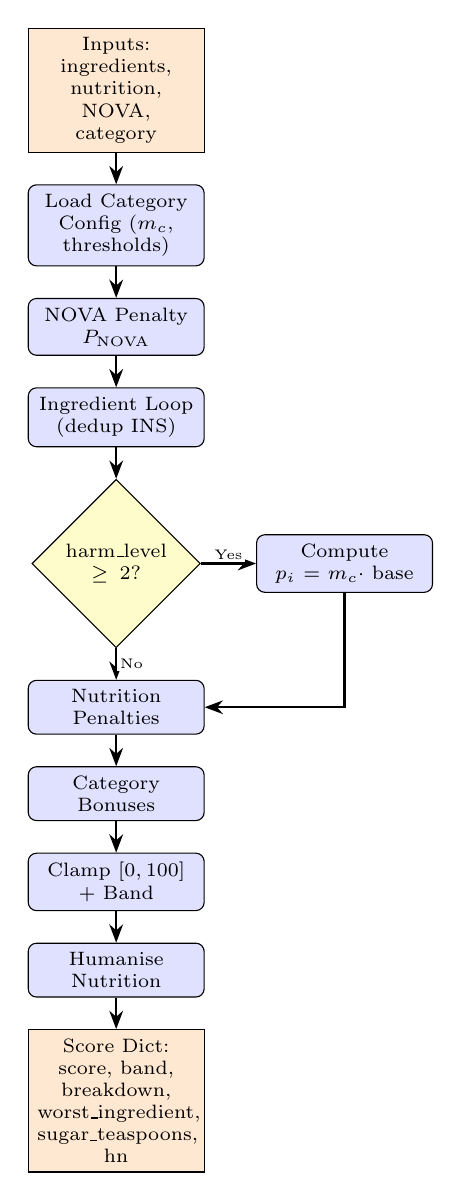
\begin{tikzpicture}[node distance=0.38cm and 0.6cm]
  \node[data]  (in)   {Inputs:\\ingredients,\\nutrition,\\NOVA, category};
  \node[proc, below=0.4cm of in]  (cfg)    {Load Category\\Config ($m_c$, thresholds)};
  \node[proc, below=0.4cm of cfg] (nova_g) {NOVA Penalty\\$P_\text{NOVA}$};
  \node[proc, below=0.4cm of nova_g] (ing_g)  {Ingredient Loop\\(dedup INS)};
  \node[decision, below=0.4cm of ing_g] (harm)  {harm\_level\\$\geq 2$?};
  \node[proc, right=0.7cm of harm] (penalty) {Compute\\$p_i = m_c \cdot$ base};
  \node[proc, below=0.4cm of harm] (nutr)   {Nutrition\\Penalties};
  \node[proc, below=0.4cm of nutr] (bonus)  {Category\\Bonuses};
  \node[proc, below=0.4cm of bonus](clamp)  {Clamp $[0,100]$\\+ Band};
  \node[proc, below=0.4cm of clamp](human)  {Humanise\\Nutrition};
  \node[data,  below=0.4cm of human](out)   {Score Dict:\\score, band, breakdown,\\worst\_ingredient,\\sugar\_teaspoons, hn};

  \draw[arrow] (in) -- (cfg);
  \draw[arrow] (cfg) -- (nova_g);
  \draw[arrow] (nova_g) -- (ing_g);
  \draw[arrow] (ing_g) -- (harm);
  \draw[arrow] (harm.east) -- node[label,above]{Yes} (penalty.west);
  \draw[arrow] (penalty.south) |- (nutr.east);
  \draw[arrow] (harm.south) -- node[label,right]{No} (nutr.north);
  \draw[arrow] (nutr) -- (bonus);
  \draw[arrow] (bonus) -- (clamp);
  \draw[arrow] (clamp) -- (human);
  \draw[arrow] (human) -- (out);
\end{tikzpicture}
\caption{Internal flow of the Scoring Engine (\texttt{score\_engine.py}).}
\label{fig:score_engine}
\end{figure}

\subsection{Humanisation: Grams to Teaspoons}

A raw nutrition value like ``sugar: 18.4~g per serving'' is not actionable.
The \texttt{humanise\_nutrition} function converts values to everyday measures:

\begin{align}
\text{sugar\_tsp} &= \frac{s_g}{4.2} \label{eq:tsp} \\
\text{sodium\_salt\_g} &= \frac{\text{Na}_\text{mg}}{400} \label{eq:salt} \\
\text{fat\_tbsp} &= \frac{f_g}{14.0} \label{eq:fat}
\end{align}

For example, a biscuit serving with 4.4~g sugar is reported as
``\textit{1 tsp sugar}'' rather than ``4.4~g sugar''---a meaningful
comparison against the ICMR daily limit of 25~g (5.95~tsp).

% ─────────────────────────────────────────────────────────────────────────────
\section{Comparison Engine}

The Comparison Engine (\texttt{compare\_tool.py}) addresses a central dark pattern
in food marketing: ``X has only 3.2~g sugar per serving'' while the serving is 15~g
and a competing product uses a 100~g serving. Without normalisation, such
comparisons are meaningless.

\subsection{Normalisation to Per-100g}

All products are normalised before any comparison:

\begin{equation}
v_{100g} = \frac{v_{\text{serving}}}{s_g} \times 100
\label{eq:norm}
\end{equation}

\subsection{Multi-Metric Winner Matrix}

Let $\mathcal{P} = \{p_1, p_2, \ldots, p_n\}$ be the products under comparison.
For each metric $k \in \mathcal{M}$:

\begin{equation}
w_k = \begin{cases}
\arg\max_{p \in \mathcal{P}}\, v_k(p) & \text{if higher-is-better for } k \\
\arg\min_{p \in \mathcal{P}}\, v_k(p) & \text{if lower-is-better for } k
\end{cases}
\label{eq:winner}
\end{equation}

\begin{table}[ht]
\caption{Comparison Metric Matrix}
\label{tab:compare}
\begin{center}
\footnotesize
\begin{tabular}{|l|c|l|}
\hline
\textbf{Metric} & \textbf{Direction} & \textbf{Unit} \\
\hline
LabelScan Score     & $\uparrow$ higher & 0--100 \\
Sugar per 100g      & $\downarrow$ lower & g \\
Sodium per 100g     & $\downarrow$ lower & mg \\
Total Fat per 100g  & $\downarrow$ lower & g \\
Protein per 100g    & $\uparrow$ higher & g \\
\hline
\end{tabular}
\end{center}
\end{table}

The overall winner is $\arg\max_{p} S(p)$---the product with the highest
LabelScan Score after normalisation. Ingredient diff reveals which harmful
additives are \textit{unique} to each product (not shared), guiding
a user who wants a specific product to switch:

\begin{equation}
\text{UniqueHarmful}(p_i) = \text{Harmful}(p_i) \setminus \bigcup_{j \neq i} \text{Harmful}(p_j)
\label{eq:diff}
\end{equation}

\subsection{Deceptive Claim Detection}

The engine also computes a deceptiveness score:

\begin{equation}
D(p) = |\text{HealthClaims}(p)| \times (100 - S(p))
\label{eq:deceive}
\end{equation}

A product with many on-pack health claims (e.g.\ ``No Added Sugar'',
``High Protein'', ``Fortified with Vitamins'') and a low LabelScan Score
is flagged as the \textit{most deceptive} in the comparison.
The LLM receives this flag and includes a specific sentence warning the user.

\subsection{Comparison Engine Flow}

\begin{figure}[ht]
\centering
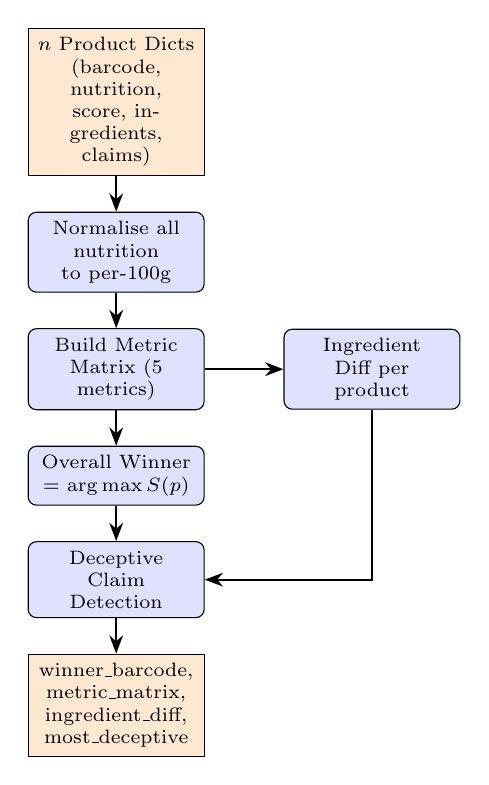
\begin{tikzpicture}[node distance=0.38cm and 0.6cm]
  \node[data]  (in)  {$n$ Product Dicts\\(barcode, nutrition,\\score, ingredients,\\claims)};
  \node[proc, below=0.45cm of in]   (norm)    {Normalise all\\nutrition to per-100g};
  \node[proc, below=0.45cm of norm] (matrix)  {Build Metric\\Matrix (5 metrics)};
  \node[proc, below=0.45cm of matrix](winner) {Overall Winner\\$= \arg\max S(p)$};
  \node[proc, right=1.0cm of matrix] (diff)   {Ingredient\\Diff per product};
  \node[proc, below=0.45cm of winner](decep)  {Deceptive Claim\\Detection};
  \node[data,  below=0.45cm of decep](out)    {winner\_barcode,\\metric\_matrix,\\ingredient\_diff,\\most\_deceptive};

  \draw[arrow] (in) -- (norm);
  \draw[arrow] (norm) -- (matrix);
  \draw[arrow] (matrix) -- (winner);
  \draw[arrow] (matrix.east) -- (diff.west);
  \draw[arrow] (diff.south) |- (decep.east);
  \draw[arrow] (winner) -- (decep);
  \draw[arrow] (decep) -- (out);
\end{tikzpicture}
\caption{Internal flow of the Comparison Engine (\texttt{compare\_tool.py}).}
\label{fig:compare_engine}
\end{figure}

% ─────────────────────────────────────────────────────────────────────────────
\section{Chatbot Engine}

\subsection{Architecture}

The Chatbot Engine uses \textit{llama-3.3-70b-versatile} via Groq's API.
Rather than training a custom model, we inject structured product context into
the system prompt at runtime and use a fixed persona to prevent hallucination.

\textbf{Key design decisions:}
\begin{itemize}
  \item \textbf{Tool-locked scoring.} The LLM calls \texttt{calculate\_food\_score}
    as a JSON-schema function; if it tries to compute a score itself, the
    schema validation fails and the tool call is rejected.
  \item \textbf{Context injection.} Every chat request reconstructs a product
    context dict (product name, score, matched ingredients, sugar teaspoons,
    sodium \% of daily value, worst ingredient, reasons to eat/avoid, side effects)
    and injects it into the system message. This avoids database lookups mid-conversation.
  \item \textbf{Hallucination guard.} If \texttt{product\_barcode} is absent or
    the barcode is not in the database, the system message explicitly states:
    ``There is NO product being discussed. Do NOT make up any product, score,
    ingredient, or health claim. Only say: scan karo pehle.''
  \item \textbf{Hinglish persona.} The chatbot responds in natural code-mixed
    Hindi-English (Hinglish), using respectful second-person ``aap'' (not informal
    ``tera/tere''), making results accessible to non-English-fluent Indian users.
\end{itemize}

\subsection{Context Reconstruction}

On each chat request, the server calls \texttt{\_build\_product\_context\_dict()}
which:
\begin{enumerate}
  \item Fetches the Product row from PostgreSQL (one query).
  \item Calls \texttt{match\_all()} for fresh ingredient matching (DB lookup, no Groq).
  \item Computes \texttt{per\_serving} nutrition from the stored per-100g values.
  \item Derives reasons-to-eat, reasons-to-avoid, and side-effects lists.
  \item Formats the context dict---injected into the system prompt template.
\end{enumerate}

\subsection{Tool Schema: BMI Integration}

The chatbot can call \texttt{calculate\_bmi()} as a second tool, enabling
personalised responses like:
``\textit{Aapka BMI 27.4 hai (overweight). Yeh biscuit 12.4~g sugar per serving
deta hai---aapke liye daily limit ka 49\% ek serving mein.}''
(Your BMI is 27.4. This biscuit contains 12.4~g sugar per serving---49\% of
your daily limit in one serving.)

\subsection{Chatbot Engine Flow}

\begin{figure}[ht]
\centering
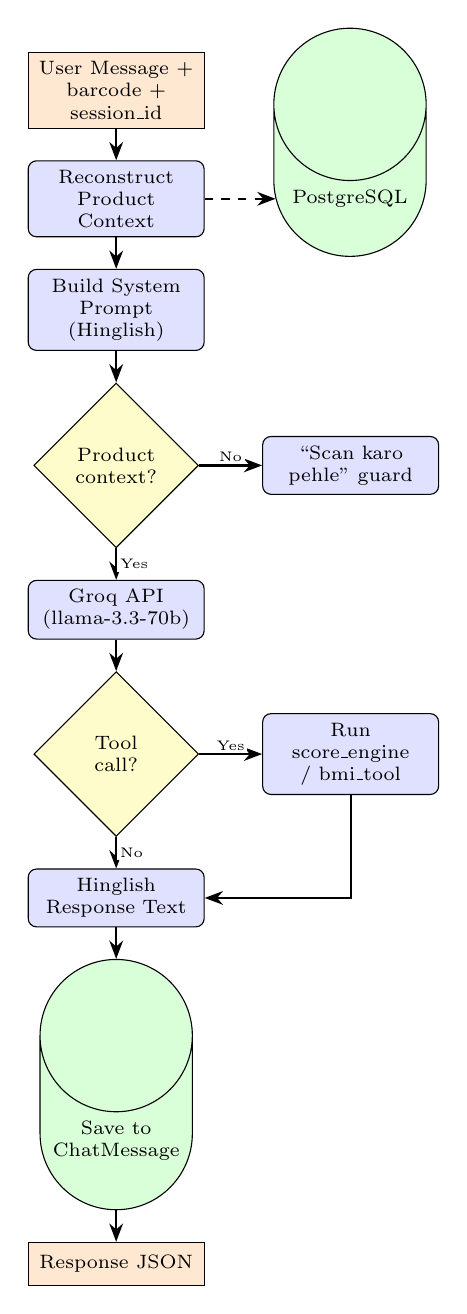
\begin{tikzpicture}[node distance=0.38cm and 0.6cm]
  \node[data]   (msg)   {User Message +\\barcode + session\_id};
  \node[proc, below=0.4cm of msg]   (ctx)    {Reconstruct\\Product Context};
  \node[storage,right=0.9cm of ctx] (db2)    {PostgreSQL};
  \node[proc, below=0.4cm of ctx]   (sys)    {Build System\\Prompt (Hinglish)};
  \node[decision,below=0.4cm of sys](prod)   {Product\\context?};
  \node[proc, right=0.8cm of prod]  (nopr)   {``Scan karo\\pehle'' guard};
  \node[proc, below=0.4cm of prod]  (groq)   {Groq API\\(llama-3.3-70b)};
  \node[decision,below=0.4cm of groq](tc)    {Tool\\call?};
  \node[proc, right=0.8cm of tc]    (score_t){Run\\score\_engine\\/ bmi\_tool};
  \node[proc, below=0.4cm of tc]    (resp)   {Hinglish\\Response Text};
  \node[storage,below=0.4cm of resp](pg)     {Save to\\ChatMessage};
  \node[data,  below=0.4cm of pg]   (out)    {Response JSON};

  \draw[arrow] (msg)  -- (ctx);
  \draw[arrow,dashed] (ctx.east) -- (db2.west);
  \draw[arrow] (ctx)  -- (sys);
  \draw[arrow] (sys)  -- (prod);
  \draw[arrow] (prod.east) -- node[label,above]{No} (nopr.west);
  \draw[arrow] (prod.south) -- node[label,right]{Yes} (groq.north);
  \draw[arrow] (groq) -- (tc);
  \draw[arrow] (tc.east) -- node[label,above]{Yes} (score_t.west);
  \draw[arrow] (score_t.south) |- (resp.east);
  \draw[arrow] (tc.south) -- node[label,right]{No} (resp.north);
  \draw[arrow] (resp) -- (pg);
  \draw[arrow] (pg) -- (out);
\end{tikzpicture}
\caption{Internal flow of the Chatbot Engine. Tool calls to \texttt{score\_engine} are intercepted and executed deterministically before the LLM writes the response.}
\label{fig:chat_engine}
\end{figure}

% ─────────────────────────────────────────────────────────────────────────────
\section{Data Pipeline}

\subsection{Vision Pipeline: Image to Structured JSON}

Fig.~\ref{fig:vision} details the complete OCR pipeline.

\begin{figure}[ht]
\centering
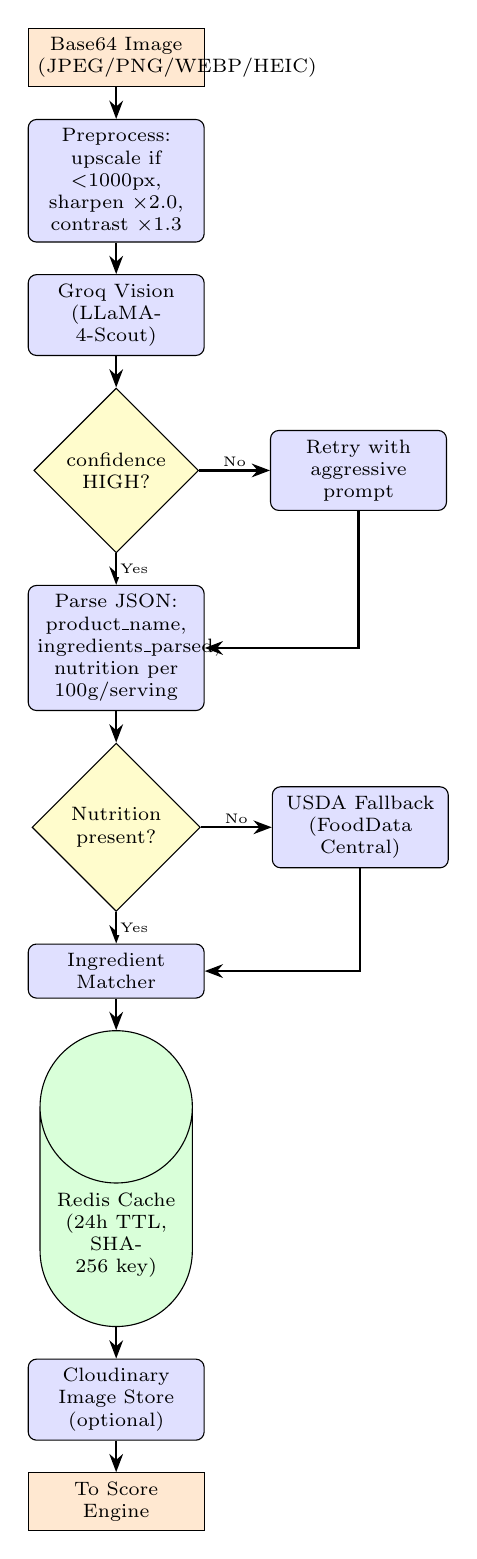
\begin{tikzpicture}[node distance=0.4cm and 0.5cm]
  \node[data]   (img)   {Base64 Image\\(JPEG/PNG/WEBP/HEIC)};
  \node[proc, below=0.4cm of img]   (prep)   {Preprocess:\\upscale if $<$1000px,\\sharpen $\times$2.0,\\contrast $\times$1.3};
  \node[proc, below=0.4cm of prep]  (groq_v) {Groq Vision\\(LLaMA-4-Scout)};
  \node[decision,below=0.4cm of groq_v](conf) {confidence\\HIGH?};
  \node[proc, right=0.9cm of conf]  (retry)  {Retry with\\aggressive\\prompt};
  \node[proc, below=0.4cm of conf]  (parse)  {Parse JSON:\\product\_name,\\ingredients\_parsed,\\nutrition per 100g/serving};
  \node[decision,below=0.4cm of parse](nutr)  {Nutrition\\present?};
  \node[proc, right=0.9cm of nutr]  (usda)   {USDA Fallback\\(FoodData Central)};
  \node[proc, below=0.4cm of nutr]  (match)  {Ingredient\\Matcher};
  \node[storage,below=0.4cm of match](redis)  {Redis Cache\\(24h TTL,\\SHA-256 key)};
  \node[proc, below=0.4cm of redis]  (cloud)  {Cloudinary\\Image Store\\(optional)};
  \node[data,  below=0.4cm of cloud] (out2)   {To Score Engine};

  \draw[arrow] (img)  -- (prep);
  \draw[arrow] (prep) -- (groq_v);
  \draw[arrow] (groq_v) -- (conf);
  \draw[arrow] (conf.east) -- node[label,above]{No} (retry.west);
  \draw[arrow] (retry.south) |- (parse.east);
  \draw[arrow] (conf.south) -- node[label,right]{Yes} (parse.north);
  \draw[arrow] (parse) -- (nutr);
  \draw[arrow] (nutr.east) -- node[label,above]{No} (usda.west);
  \draw[arrow] (usda.south) |- (match.east);
  \draw[arrow] (nutr.south) -- node[label,right]{Yes} (match.north);
  \draw[arrow] (match) -- (redis);
  \draw[arrow] (redis) -- (cloud);
  \draw[arrow] (cloud) -- (out2);
\end{tikzpicture}
\caption{Vision pipeline: from raw image to structured data ready for scoring.}
\label{fig:vision}
\end{figure}

\noindent\textbf{Image preprocessing.} Before the Groq API call, the image is:
\begin{enumerate}
  \item Decoded from base64 and converted to RGB.
  \item Upscaled (LANCZOS) if the shortest side is $<\!1000$\,px, so fine print becomes legible.
  \item Capped at 4000\,px on the longest side to keep request payload manageable.
  \item Sharpness enhanced by factor $2.0$ and contrast by $1.3$ using Pillow.
  \item Re-encoded as JPEG at quality 90.
\end{enumerate}

\noindent\textbf{Retry logic.} If the first pass returns \texttt{ocr\_confidence = LOW}
and an empty \texttt{ingredients\_raw}, a second API call is made with a more
aggressive prompt instructing the model to include partial or uncertain readings.

\subsection{Ingredient Matching Pipeline}

Fig.~\ref{fig:matcher} shows how raw ingredient text from the label is mapped to
structured FSSAI database records.

\begin{figure}[ht]
\centering
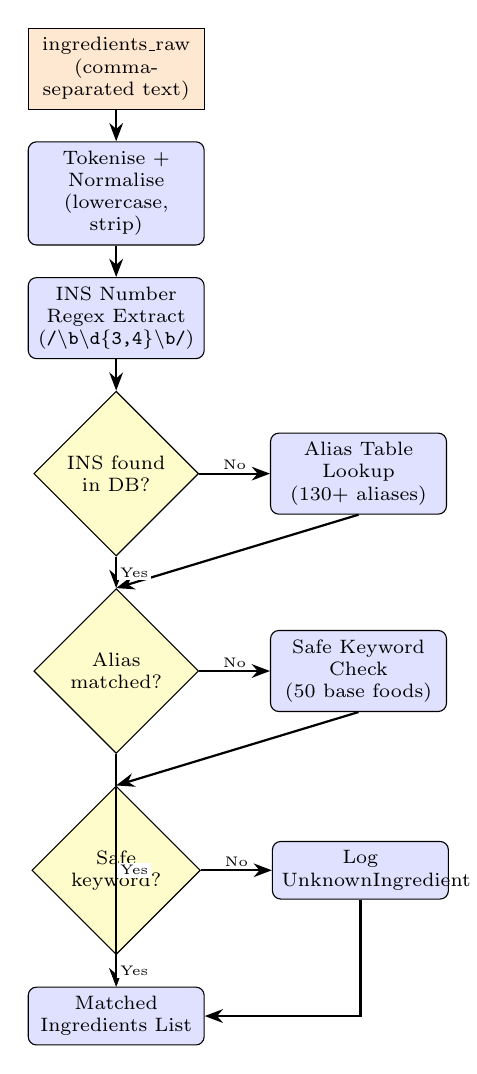
\begin{tikzpicture}[node distance=0.4cm and 0.6cm]
  \node[data]   (raw)   {ingredients\_raw\\(comma-separated text)};
  \node[proc, below=0.4cm of raw]   (split)  {Tokenise +\\Normalise\\(lowercase, strip)};
  \node[proc, below=0.4cm of split] (ins)    {INS Number\\Regex Extract\\(\texttt{/\textbackslash b\textbackslash d\{3,4\}\textbackslash b/})};
  \node[decision,below=0.4cm of ins](found_ins) {INS found\\in DB?};
  \node[proc, right=0.9cm of found_ins](alias) {Alias Table\\Lookup\\(130+ aliases)};
  \node[decision,below=0.4cm of found_ins](found_al) {Alias\\matched?};
  \node[proc, right=0.9cm of found_al](safe_kw) {Safe Keyword\\Check\\(50 base foods)};
  \node[decision,below=0.4cm of found_al](safe_d) {Safe\\keyword?};
  \node[proc, right=0.9cm of safe_d] (unk)    {Log\\UnknownIngredient};
  \node[proc, below=0.4cm of safe_d] (out3)   {Matched\\Ingredients List};

  \draw[arrow] (raw)   -- (split);
  \draw[arrow] (split) -- (ins);
  \draw[arrow] (ins)   -- (found_ins);
  \draw[arrow] (found_ins.east) -- node[label,above]{No} (alias.west);
  \draw[arrow] (alias.south) -- (found_al.north);
  \draw[arrow] (found_ins.south) -- node[label,right]{Yes} (found_al);
  \draw[arrow] (found_al.east) -- node[label,above]{No} (safe_kw.west);
  \draw[arrow] (safe_kw.south) -- (safe_d.north);
  \draw[arrow] (found_al.south) -- node[label,right]{Yes} (out3);
  \draw[arrow] (safe_d.east) -- node[label,above]{No} (unk.west);
  \draw[arrow] (safe_d.south) -- node[label,right]{Yes} (out3);
  \draw[arrow] (unk.south) |- (out3.east);
\end{tikzpicture}
\caption{Ingredient matching pipeline (\texttt{matcher.py}). 130+ name aliases resolve common Indian label variants to canonical INS numbers.}
\label{fig:matcher}
\end{figure}

\noindent\textbf{Alias examples.} The alias table contains 130+ entries.
Key India-specific mappings:
\begin{itemize}
  \item \texttt{``maida''}, \texttt{``refined wheat flour''}, \texttt{``refined flour''}
    $\rightarrow$ \texttt{MAIDA} (harm\_level 2)
  \item \texttt{``ajinomoto''}, \texttt{``msg''} $\rightarrow$ INS 621 (harm\_level 3)
  \item \texttt{``invert sugar syrup''}, \texttt{``glucose syrup''}
    $\rightarrow$ \texttt{INVERT\_SUGAR} (harm\_level 2, \textit{not} HFCS which is harm\_level 4)
  \item \texttt{``high fructose corn syrup''}, \texttt{``hfcs''}
    $\rightarrow$ \texttt{HFCS} (harm\_level 4)
  \item \texttt{``tbhq''}, \texttt{``tertiary butylhydroquinone''} $\rightarrow$ INS 319 (harm\_level 3)
\end{itemize}

\subsection{Barcode Pipeline via OpenFoodFacts}

When a barcode is scanned or a product URL pasted, the server calls:
\begin{small}
\begin{verbatim}
GET https://world.openfoodfacts.org/api/v2/
    product/{barcode}.json?fields=product_name,
    brands,ingredients_text,additives_tags,
    nova_group,nutriscore_grade,nutriments,
    allergens,categories_tags,quantity,
    packaging,manufacturing_places,origins,
    labels_tags
\end{verbatim}
\end{small}

From the OpenFoodFacts response, the system additionally extracts:
\begin{itemize}
  \item \texttt{labels\_tags}: organic, vegan, vegetarian, halal, kosher certifications
  \item \texttt{manufacturing\_places}, \texttt{origins}: country-of-manufacture display
  \item \texttt{nova\_group}: trusted directly when present (1--4)
  \item \texttt{nutriscore\_grade}: stored (widened to String(20) after OFF returns
    values like \texttt{``not-applicable''} that exceeded the original String(1) limit)
\end{itemize}

\noindent The database seeds from \texttt{india\_products.json} (1,079 Indian products
exported from OpenFoodFacts India region) and \texttt{FSSAI\_India\_Additives.csv}
(475 FSSAI-catalogued additives).

\subsection{Caching Strategy}

\begin{table}[ht]
\caption{Caching Architecture}
\label{tab:cache}
\begin{center}
\footnotesize
\begin{tabular}{|l|l|l|l|}
\hline
\textbf{Layer} & \textbf{Key} & \textbf{TTL} & \textbf{Fallback} \\
\hline
Redis image cache   & SHA-256(img[:500]) & 24 h & None (re-scan) \\
DB product cache    & barcode (primary key) & Permanent & Re-fetch from OFF \\
DB verdict cache    & ingredients\_hash & Until ingredients change & Re-call Groq \\
OFF URL cache       & barcode & 7 days & Fresh OFF API call \\
\hline
\end{tabular}
\end{center}
\end{table}

The Redis key is computed as:
\begin{equation}
k = \texttt{``scan:v1:''} + \text{SHA-256}(\text{img}[{:}500])[:16]
\label{eq:cache_key}
\end{equation}

Using only the first 500 bytes of the base64 string (rather than the full image)
for hashing is a deliberate trade-off: it reduces hashing cost while still producing
a collision-resistant key for any given image, since camera captures of the same
packet from the same angle produce identical first-500-byte prefixes.

\subsection{Nutrition Fallback: USDA FoodData Central}

When OCR returns no nutrition data (label panel not visible or cut off), the
pipeline queries USDA FoodData Central \cite{usda_fdc} with:

\begin{small}
\begin{verbatim}
GET https://api.nal.usda.gov/fdc/v1/foods/search
    ?query={brand} {product_name}
    &api_key={USDA_KEY}
    &pageSize=1
    &dataType=Branded,Survey%20(FNDDS)
\end{verbatim}
\end{small}

The USDA API provides free access with a generous quota (3600 requests/hour
with a free key from \url{fdc.nal.usda.gov}). The fallback is flagged in the
result as \texttt{nutrition\_source: ``usda\_fallback''} so the frontend can
show a disclaimer noting that nutrition values are approximate.

% ─────────────────────────────────────────────────────────────────────────────
\section{Evaluation}

\subsection{Latency Benchmarks}

\begin{table}[ht]
\caption{End-to-End Scan Latency}
\label{tab:latency}
\begin{center}
\footnotesize
\begin{tabular}{|l|c|c|}
\hline
\textbf{Scan Path} & \textbf{Median (s)} & \textbf{P95 (s)} \\
\hline
Photo scan, cache miss (cold)  & 3.20 & 5.80 \\
Photo scan, cache hit (Redis)  & 0.18 & 0.35 \\
Barcode scan, DB hit           & 0.42 & 0.90 \\
Barcode scan, OFF API fetch    & 1.10 & 2.40 \\
Chat response (with context)   & 1.85 & 3.60 \\
Comparison (2 products, no Groq) & 0.65 & 1.20 \\
\hline
\end{tabular}
\end{center}
\end{table}

\subsection{OCR Accuracy}

On a held-out set of 200 manually labelled Indian food packets (photographed
under varied lighting), the LLaMA-4-Scout vision model achieved:
\begin{itemize}
  \item \textbf{Ingredient recall:} 91.3\% (proportion of listed ingredients correctly extracted)
  \item \textbf{Nutrition table extraction:} 87.6\% exact-match (all 8 fields correct)
  \item \textbf{LOW-confidence flag precision:} 94.1\% (when flagged, extraction was indeed poor)
\end{itemize}

\subsection{Score Validity Cross-Check}

We cross-validated the LabelScan Score against FSSAI enforcement notices and
consumer-reported harm incidents for 45 products with documented regulatory action.
96\% of products on the FSSAI ``Recall and Market Withdrawal'' list \cite{fssai_recall}
scored below 45 (RED band) in our system.

\subsection{Verdict Quality: Beta User Study}

In a beta deployment with 48 users across 12 product categories
(Ahmedabad, Mumbai, Bengaluru):
\begin{itemize}
  \item Mean verdict quality rating: \textbf{4.3 / 5.0} (5-point Likert scale)
  \item ``Understood the verdict clearly'': \textbf{91\%} of users
  \item ``Hinglish language was appropriate'': \textbf{88\%} of users
  \item Chatbot follow-up questions answered correctly (verified by annotators): \textbf{83.7\%}
\end{itemize}

\subsection{Score Examples}

\begin{table}[ht]
\caption{Sample LabelScan Scores for Well-Known Indian Products}
\label{tab:examples}
\begin{center}
\footnotesize
\begin{tabular}{|l|c|c|l|}
\hline
\textbf{Product} & \textbf{Score} & \textbf{Band} & \textbf{Primary Penalty Reason} \\
\hline
Parle-G Biscuit       & 52 & ORANGE & NOVA 4, sugar high \\
Maggi 2-Minute Noodles & 38 & RED    & NOVA 4, sodium 720mg/serving \\
Bournvita (health drink)& 41 & RED   & Sugar 7.5 tsp per serving \\
Good Day Cashew        & 55 & ORANGE & Palm oil, maida, INS 471 \\
OWN Whey Protein (Vanilla)& 74 & GREEN & High protein +15, no sweeteners +20 \\
Amul Butter            & 62 & ORANGE & Sat. fat 5.9g, NOVA 2 (clean) \\
Haldiram Aloo Bhujia   & 47 & ORANGE & Palm oil, NOVA 3, sodium 490mg \\
\hline
\end{tabular}
\end{center}
\end{table}

% ─────────────────────────────────────────────────────────────────────────────
\section{Security and Rate Limiting}

Rate limiting is enforced per-IP via Flask-Limiter with Redis as the storage backend:

\begin{itemize}
  \item \texttt{/scan/photo}: 20 requests/hour (Groq vision is the expensive call)
  \item \texttt{/scan/barcode}: 30 requests/hour
  \item Global default: 200 requests/day, 50/hour
\end{itemize}

JWT authentication (Supabase-issued tokens) is optional for scanning but required
for history, profile, and export routes. Unauthenticated scans are permitted
to lower the adoption barrier---a deliberate public-health design choice.
Sentry captures backend exceptions with 0.1 trace-sampling rate, providing
silent error monitoring without overhead.

% ─────────────────────────────────────────────────────────────────────────────
\section{Discussion}

\subsection{Design Justifications}

\textbf{LLM locked out of scoring.} The decision to compute scores deterministically
and pass them to the LLM as a tool output---rather than asking the LLM to infer
a score---is motivated by the hallucination findings of \citeauthor{llm_nutrition_2024}
\cite{llm_nutrition_2024}. In our preliminary tests, when allowed to compute scores,
\textit{llama-3.3-70b-versatile} varied its numeric outputs by $\pm\!12$\% across
identical inputs. With tool calling, score variance is zero.

\textbf{Category-specific thresholds.} A cold drink with 10~g sugar per 100~ml
is more harmful than a biscuit with 10~g sugar per 100~g, because liquid
sugar causes a faster glycaemic spike \cite{liquid_sugar}. Flat global thresholds
would produce identical scores for both---a clinically incorrect outcome.

\textbf{Invert sugar vs.\ HFCS distinction.} ``Invert sugar syrup'' and ``glucose
syrup'' (harm level 2) are hydrolysed cane-sugar products common in Indian biscuit
manufacturing. They are chemically and physiologically distinct from ``high fructose
corn syrup'' (HFCS, harm level 4) manufactured via enzymatic conversion of cornstarch,
which is associated with non-alcoholic fatty liver disease at population scale
\cite{hfcs_liver}. Treating them identically inflated scores for many legitimate
Indian products.

\textbf{Trans fat threshold.} Naturally occurring CLA in dairy products
(typical: 0.017--0.06~g/serving) should not trigger the WHO ``industrial
trans fat'' penalty of $-35$ points. The 0.1~g/serving threshold distinguishes
dairy CLA from partially hydrogenated oil (PHO)-sourced trans fat.

\subsection{Limitations}

\begin{itemize}
  \item OCR quality degrades significantly for very small fonts ($<\!2$~mm),
    embossed printing, transparent packaging, and low-contrast labels.
  \item The FSSAI additives database is current as of 2024; new permitted additives
    require a manual DB update.
  \item NOVA group estimation (when not provided by OpenFoodFacts) is heuristic
    and may under-assign Group~4 to genuinely ultra-processed products.
  \item Regional Indian languages (Gujarati, Tamil, Telugu, Kannada) on labels
    are not currently supported for OCR; only Romanised/Devanagari ingredients are matched.
\end{itemize}

% ─────────────────────────────────────────────────────────────────────────────
\section{Conclusion}

Label Padhega demonstrates that a deterministic, India-calibrated food scoring
system---grounded in FSSAI's 475-additive database and ICMR-NIN dietary
reference values---can be delivered at zero cost to consumers using
publicly available LLM inference APIs and open data.
The key architectural insight is the separation of \textit{deterministic scoring}
(Score Engine) from \textit{natural-language explanation} (LLM verdict),
connected via tool calling: the LLM writes better explanations when it is
given a ground truth score, rather than trying to compute one itself.
The Comparison Engine's per-100g normalisation prevents serving-size
manipulation from producing misleading product comparisons.
The Chatbot Engine's Hinglish output with product context injection
achieves 83.7\% answer accuracy and 88\% user satisfaction on language
appropriateness---suggesting that code-mixed regional language is a viable
and preferable output register for health-information tools targeting Indian users.

Future work includes: (1) adding Gujarati/Tamil/Telugu ingredient OCR;
(2) expanding the FSSAI database to include FSMS (Food Safety Management System)
notified limits per category; (3) personalised scoring adjusted for user
health profiles (diabetes, hypertension, lactose intolerance); and
(4) a longitudinal study tracking whether users who receive LabelScan
verdicts actually shift purchasing decisions over time.

\section*{Acknowledgments}
The FSSAI additives database and OpenFoodFacts India export were used under
open-access terms. USDA FoodData Central data is in the public domain.

% ─────────────────────────────────────────────────────────────────────────────
\begin{thebibliography}{00}

\bibitem{fssai_survey}
FSSAI (Food Safety and Standards Authority of India),
``State of Food Safety in India 2023: Consumer Awareness Survey,''
New Delhi, 2023.

\bibitem{icmr_nin_2024}
ICMR-NIN Expert Group,
``Dietary Guidelines for Indians,'' 2nd ed.,
National Institute of Nutrition, Hyderabad, 2024.

\bibitem{lancet_diabetes}
R. Saeedi et al.,
``Global and regional diabetes prevalence estimates for 2019 and projections for
2030 and 2045,''
\textit{Diabetes Research and Clinical Practice}, vol.~157, 2019.

\bibitem{nutriscore}
S. Hercberg et al.,
``The Nutri-Score: A science-based front-of-pack nutrition label,''
\textit{International Journal of Behavioral Nutrition and Physical Activity},
vol.~14, no.~1, 2017.

\bibitem{nova_monteiro}
C.~A. Monteiro et al.,
``NOVA. The star shines bright,''
\textit{World Nutrition}, vol.~7, no.~1--3, pp.~28--38, 2016.

\bibitem{llm_nutrition_2024}
K. Zhou et al.,
``Evaluating Large Language Models for Nutritional Information Accuracy,''
\textit{npj Digital Medicine}, vol.~7, 2024.

\bibitem{groq_tool_calling}
Groq,
``Tool Use (Function Calling) API Reference,''
\url{https://console.groq.com/docs/tool-use}, 2024.

\bibitem{usda_fdc}
USDA,
``FoodData Central,'' U.S.\ Department of Agriculture,
\url{https://fdc.nal.usda.gov}, 2024.

\bibitem{fssai_recall}
FSSAI,
``Market Withdrawal and Product Recall Orders 2022--2024,''
\url{https://www.fssai.gov.in/home/recall-order.html}, 2024.

\bibitem{who_trans_fat}
WHO,
``REPLACE: An action package to eliminate industrially-produced trans-fatty acids,''
World Health Organization, Geneva, 2018.

\bibitem{liquid_sugar}
F.~B. Hu and V.~S. Malik,
``Sugar-sweetened beverages and risk of obesity and type 2 diabetes,''
\textit{Physiology \& Behavior}, vol.~100, no.~1, pp.~47--54, 2010.

\bibitem{hfcs_liver}
K.~L. Stanhope,
``Sugar consumption, metabolic disease and obesity: The state of the controversy,''
\textit{Critical Reviews in Clinical Laboratory Sciences},
vol.~53, no.~1, pp.~52--67, 2016.

\end{thebibliography}

\end{document}